\section{Augmenting odd arrangements}\label{sec:augment}

We continue with ways to obtain arrangements of an even number of pseudolines, now by adding one pseudoline to a triangle-maximal odd arrangement.

\subsection{Augmentation by an outermost line}

Even arrangements of straight lines with the largest known number of triangles are often obtained by adding one line that passes far from all intersection points~\cite{bbl,blanc11,savchuk25}. We call such a line \emph{outermost}. A perfect arrangement of $n$ lines, $n\equiv3,5\pmod 6$, has $n(n-2)/3$ triangles and $n$ external digons~\cite[Lemma~2.3]{pu26b}.
The outermost line crosses both sides of $(n-1)/2$ external digons and cuts off a new triangle from each of them (see \cref{fig:outermost} for pseudolines).
The new simple arrangement $\mathcal{A}$ of $N=n+1$ lines therefore has
\[
a_3(\mathcal{A})=\frac{n(n-2)}3+\frac{n-1}2=\frac{N(2N-5)}6
\]
triangles, so it attains the bound \eqref{eq:blanc-even}.

\begin{figure}[H]
\centering
\tikzset{every picture/.append style={yscale=0.71}}
\begin{minipage}{0.85\linewidth}
% Generated by Visual Arnold
\begin{tikzpicture}[x=\linewidth,y=\linewidth,
  poly/.style={fill=gray!20},
  ext/.style={black,line width=0.3pt},
  aug/.style={r-line,thick,dashed,line cap=round,line join=round},
  lbl/.style={inner sep=0pt,font=\scriptsize},
  plbl/.style={inner sep=0pt,font=\scriptsize}]
\useasboundingbox (0,0) rectangle (1,-0.78947);
\clip (0,0) rectangle (1,-0.78947);
\fill[poly] (0.67839,-0.21093) -- (0.78893,-0.10133) -- (0.75874,-0.20389) -- cycle;
\fill[poly] (0.54269,-0.23377) -- (0.55397,-0.07990) -- (0.58838,-0.22267) -- cycle;
\fill[poly] (0.41293,-0.29891) -- (0.33541,-0.13233) -- (0.49173,-0.25367) -- cycle;
\fill[poly] (0.44394,-0.36827) -- (0.36979,-0.33229) -- (0.41293,-0.29891) -- cycle;
\fill[poly] (0.53946,-0.29355) -- (0.49173,-0.25367) -- (0.54269,-0.23377) -- cycle;
\fill[poly] (0.59971,-0.28967) -- (0.58838,-0.22267) -- (0.67839,-0.21093) -- cycle;
\fill[poly] (0.53810,-0.35967) -- (0.53946,-0.29355) -- (0.56988,-0.32215) -- cycle;
\fill[poly] (0.47912,-0.44083) -- (0.44394,-0.36827) -- (0.50530,-0.40260) -- cycle;
\fill[poly] (0.53885,-0.42341) -- (0.50530,-0.40260) -- (0.53810,-0.35967) -- cycle;
\fill[poly] (0.60661,-0.36109) -- (0.56988,-0.32215) -- (0.59971,-0.28967) -- cycle;
\fill[poly] (0.71254,-0.34584) -- (0.75874,-0.20389) -- (0.90848,-0.18950) -- cycle;
\fill[poly] (0.60999,-0.42389) -- (0.60661,-0.36109) -- (0.64017,-0.40194) -- cycle;
\fill[poly] (0.54016,-0.47171) -- (0.53885,-0.42341) -- (0.57520,-0.44880) -- cycle;
\fill[poly] (0.40823,-0.55380) -- (0.47912,-0.44083) -- (0.50863,-0.49208) -- cycle;
\fill[poly] (0.54377,-0.54287) -- (0.50863,-0.49208) -- (0.54016,-0.47171) -- cycle;
\fill[poly] (0.61242,-0.47536) -- (0.57520,-0.44880) -- (0.60999,-0.42389) -- cycle;
\fill[poly] (0.67196,-0.44612) -- (0.64017,-0.40194) -- (0.71254,-0.34584) -- cycle;
\fill[poly] (0.61557,-0.54580) -- (0.61242,-0.47536) -- (0.64473,-0.49914) -- cycle;
\fill[poly] (0.54920,-0.64080) -- (0.54377,-0.54287) -- (0.58300,-0.59264) -- cycle;
\fill[poly] (0.62258,-0.63918) -- (0.58300,-0.59264) -- (0.61557,-0.54580) -- cycle;
\fill[poly] (0.76420,-0.58473) -- (0.64473,-0.49914) -- (0.67196,-0.44612) -- cycle;
\fill[poly] (0.83820,-0.68491) -- (0.76420,-0.58473) -- (0.90664,-0.67682) -- cycle;
\fill[poly] (0.63138,-0.70965) -- (0.62258,-0.63918) -- (0.68079,-0.70621) -- cycle;
\fill[poly] (0.50810,-0.70459) -- (0.54920,-0.64080) -- (0.55281,-0.70901) -- cycle;
\fill[poly] (0.24993,-0.65307) -- (0.40823,-0.55380) -- (0.33503,-0.67147) -- cycle;
\draw[ext] (0.31573,-0.30606) -- (0.36979,-0.33229) -- (0.44394,-0.36827) -- (0.50530,-0.40260) -- (0.53885,-0.42341) -- (0.57520,-0.44880) -- (0.61242,-0.47536) -- (0.64473,-0.49914) -- (0.76420,-0.58473) -- (0.90664,-0.67682) -- (0.95710,-0.70945);
\node[lbl] at (0.30493,-0.30083) {0};
\node[lbl] at (0.96718,-0.71596) {0};
\draw[ext] (0.28794,-0.09548) -- (0.33541,-0.13233) -- (0.49173,-0.25367) -- (0.53946,-0.29355) -- (0.56988,-0.32215) -- (0.60661,-0.36109) -- (0.64017,-0.40194) -- (0.67196,-0.44612) -- (0.76420,-0.58473) -- (0.83820,-0.68491) -- (0.87390,-0.73324);
\node[lbl] at (0.27846,-0.08812) {1};
\node[lbl] at (0.88103,-0.74289) {1};
\draw[ext] (0.31006,-0.07785) -- (0.33541,-0.13233) -- (0.41293,-0.29891) -- (0.44394,-0.36827) -- (0.47912,-0.44083) -- (0.50863,-0.49208) -- (0.54377,-0.54287) -- (0.58300,-0.59264) -- (0.62258,-0.63918) -- (0.68079,-0.70621) -- (0.72018,-0.75158);
\node[lbl] at (0.30499,-0.06697) {2};
\node[lbl] at (0.72805,-0.76065) {2};
\draw[ext] (0.53989,-0.02148) -- (0.55397,-0.07990) -- (0.58838,-0.22267) -- (0.59971,-0.28967) -- (0.60661,-0.36109) -- (0.60999,-0.42389) -- (0.61242,-0.47536) -- (0.61557,-0.54580) -- (0.62258,-0.63918) -- (0.63138,-0.70965) -- (0.63882,-0.76928);
\node[lbl] at (0.53708,-0.00982) {3};
\node[lbl] at (0.64030,-0.78119) {3};
\draw[ext] (0.55836,-0.01997) -- (0.55397,-0.07990) -- (0.54269,-0.23377) -- (0.53946,-0.29355) -- (0.53810,-0.35967) -- (0.53885,-0.42341) -- (0.54016,-0.47171) -- (0.54377,-0.54287) -- (0.54920,-0.64080) -- (0.55281,-0.70901) -- (0.55598,-0.76902);
\node[lbl] at (0.55924,-0.00800) {4};
\node[lbl] at (0.55662,-0.78100) {4};
\draw[ext] (0.80590,-0.04368) -- (0.78893,-0.10133) -- (0.75874,-0.20389) -- (0.71254,-0.34584) -- (0.67196,-0.44612) -- (0.64473,-0.49914) -- (0.61557,-0.54580) -- (0.58300,-0.59264) -- (0.54920,-0.64080) -- (0.50810,-0.70459) -- (0.47556,-0.75510);
\node[lbl] at (0.80929,-0.03217) {5};
\node[lbl] at (0.46906,-0.76519) {5};
\draw[ext] (0.83160,-0.05902) -- (0.78893,-0.10133) -- (0.67839,-0.21093) -- (0.59971,-0.28967) -- (0.56988,-0.32215) -- (0.53810,-0.35967) -- (0.50530,-0.40260) -- (0.47912,-0.44083) -- (0.40823,-0.55380) -- (0.33503,-0.67147) -- (0.30329,-0.72249);
\node[lbl] at (0.84012,-0.05057) {6};
\node[lbl] at (0.29696,-0.73268) {6};
\draw[ext] (0.95545,-0.15202) -- (0.90848,-0.18950) -- (0.71254,-0.34584) -- (0.64017,-0.40194) -- (0.60999,-0.42389) -- (0.57520,-0.44880) -- (0.54016,-0.47171) -- (0.50863,-0.49208) -- (0.40823,-0.55380) -- (0.24993,-0.65307) -- (0.19902,-0.68499);
\node[lbl] at (0.96483,-0.14454) {7};
\node[lbl] at (0.18886,-0.69137) {7};
\draw[ext] (0.96829,-0.18375) -- (0.90848,-0.18950) -- (0.75874,-0.20389) -- (0.67839,-0.21093) -- (0.58838,-0.22267) -- (0.54269,-0.23377) -- (0.49173,-0.25367) -- (0.41293,-0.29891) -- (0.36979,-0.33229) -- (0.07808,-0.61673) -- (0.03506,-0.65868);
\node[lbl] at (0.98023,-0.18260) {8};
\node[lbl] at (0.02646,-0.66706) {8};
\draw[aug] (0.96632,-0.66978) -- (0.90664,-0.67682) -- (0.83820,-0.68491) -- (0.68079,-0.70621) -- (0.63138,-0.70965) -- (0.55281,-0.70901) -- (0.50810,-0.70459) -- (0.33503,-0.67147) -- (0.24993,-0.65307) -- (0.07808,-0.61673) -- (0.01929,-0.60430);
\node[lbl] at (0.97823,-0.66837) {9};
\node[lbl] at (0.00755,-0.60181) {9};
\end{tikzpicture}

\end{minipage}
\caption{A perfect arrangement of 9 pseudolines, labeled 0 to 8, and the outermost pseudoline 9 (dashed).
The resulting arrangement of 10 pseudolines has $a_3=25$ triangles.}
\label{fig:outermost}
\end{figure}

\subsection{Augmentation patterns for multiple points}\label{sec:augment-patterns}

For $n\equiv1\pmod 6$ there are no perfect arrangements. Here the triangle-maximal arrangements belong to the wider family of \emph{2-defective arrangements}. This family can be introduced as follows. Pass to the projective closure by adding the line at infinity. It consists of an even number $n+1$ of pseudolines, so its faces admit a checkerboard coloring, in which faces sharing a side get different colors. Call black the color of at least half of the faces. The black faces are the same for all affine charts of the projective arrangement, whichever of its pseudolines is sent to infinity. The non-triangular projective black faces are called \emph{defects}. For $n\equiv1\pmod 6$ the number of black faces is maximal precisely when there are either two quadrilateral defects or one pentagonal defect; such arrangements are called \emph{2-defective}~\cite[Lemma~2.7 and Definition~2.8]{pu26b}. An affine arrangement is triangle-maximal if and only if it is 2-defective and all its defects are external (unbounded)~\cite[Lemma~2.9]{pu26b}.

We now consider how 2-defective arrangements can be augmented.
An outermost line can still be added~\cite[Proposition~5.1]{blanc11}, but its position must be chosen so that it does not cross both unbounded sides of an external defect. Otherwise it cuts off fewer than $(n-1)/2$ new triangles. The result is again a simple arrangement, and the same bound \eqref{eq:blanc-even} holds for it.
We found two augmentation patterns for 2-defective arrangements that can exceed this bound.

In the first pattern, which we call \emph{direct augmentation}, the new pseudoline is drawn directly through the original 2-defective arrangement (\cref{fig:direct}). It must cut off triangles from both quadrilateral defects and close up through other sides and vertices. After a possible change of affine chart, the number of triangles can reach the value given by \eqref{eq:conj-bound}.

\begin{figure}[p]
\centering
\tikzset{every picture/.append style={yscale=0.86}}
%\tikzset{every picture/.append style={execute at end picture={\draw[red,thin] (current bounding box.south west) rectangle (current bounding box.north east);}}}% DEBUG: picture frame
\captionsetup[sub]{skip=-8pt}% gap between the picture frame and the caption; may be negative
\begin{subfigure}[b]{0.75\linewidth}
\centering
% Generated by Visual Arnold
\begin{tikzpicture}[x=\linewidth,y=\linewidth,
  poly/.style={fill=gray!20},
  defect/.style={fill=red!20},
  ext/.style={black,line width=0.3pt},
  aug/.style={r-line,thick,dashed,line cap=round,line join=round},
  lbl/.style={inner sep=0pt,font=\tiny},
  plbl/.style={inner sep=0pt,font=\tiny}]
\useasboundingbox (0,0) rectangle (1,-0.89661);
\clip (0,0) rectangle (1,-0.89661);
\fill[poly] (0.49097,-0.69175) -- (0.45162,-0.81477) -- (0.44043,-0.72291) -- cycle;
\fill[poly] (0.60266,-0.63936) -- (0.61679,-0.75904) -- (0.55336,-0.66290) -- cycle;
\fill[poly] (0.67611,-0.58225) -- (0.74524,-0.67747) -- (0.64359,-0.61285) -- cycle;
\fill[poly] (0.73836,-0.48302) -- (0.84733,-0.54944) -- (0.70743,-0.53978) -- cycle;
\fill[poly] (0.80373,-0.36240) -- (0.91295,-0.36444) -- (0.77162,-0.41542) -- cycle;
\fill[poly] (0.68806,-0.43399) -- (0.77162,-0.41542) -- (0.73836,-0.48302) -- cycle;
\fill[poly] (0.64585,-0.54131) -- (0.70743,-0.53978) -- (0.67611,-0.58225) -- cycle;
\fill[poly] (0.60388,-0.58441) -- (0.64359,-0.61285) -- (0.60266,-0.63936) -- cycle;
\fill[poly] (0.60796,-0.49770) -- (0.64585,-0.54131) -- (0.60630,-0.54418) -- cycle;
\fill[poly] (0.56895,-0.45682) -- (0.60352,-0.44978) -- (0.60796,-0.49770) -- cycle;
\fill[poly] (0.56470,-0.54916) -- (0.60630,-0.54418) -- (0.60388,-0.58441) -- cycle;
\fill[poly] (0.51312,-0.60600) -- (0.55336,-0.66290) -- (0.49097,-0.69175) -- cycle;
\fill[poly] (0.52707,-0.50886) -- (0.56470,-0.54916) -- (0.52161,-0.55426) -- cycle;
\fill[poly] (0.53755,-0.42353) -- (0.56895,-0.45682) -- (0.53208,-0.46352) -- cycle;
\fill[poly] (0.49319,-0.46913) -- (0.53208,-0.46352) -- (0.52707,-0.50886) -- cycle;
\fill[poly] (0.47885,-0.55547) -- (0.52161,-0.55426) -- (0.51312,-0.60600) -- cycle;
\fill[poly] (0.41844,-0.62976) -- (0.44043,-0.72291) -- (0.36098,-0.79258) -- cycle;
\fill[poly] (0.44718,-0.51351) -- (0.47885,-0.55547) -- (0.43887,-0.54968) -- cycle;
\fill[poly] (0.46049,-0.42998) -- (0.49319,-0.46913) -- (0.45448,-0.47407) -- cycle;
\fill[poly] (0.41750,-0.47898) -- (0.45448,-0.47407) -- (0.44718,-0.51351) -- cycle;
\fill[poly] (0.39232,-0.53120) -- (0.43887,-0.54968) -- (0.41844,-0.62976) -- cycle;
\fill[poly] (0.38394,-0.44298) -- (0.41750,-0.47898) -- (0.38409,-0.48303) -- cycle;
\fill[poly] (0.32322,-0.48984) -- (0.38409,-0.48303) -- (0.39232,-0.53120) -- cycle;
\fill[poly] (0.26943,-0.45826) -- (0.32322,-0.48984) -- (0.19192,-0.51559) -- cycle;
\fill[poly] (0.38817,-0.39609) -- (0.38394,-0.44298) -- (0.35496,-0.40719) -- cycle;
\fill[poly] (0.46564,-0.38711) -- (0.46049,-0.42998) -- (0.42648,-0.38977) -- cycle;
\fill[poly] (0.54339,-0.38644) -- (0.53755,-0.42353) -- (0.50510,-0.38652) -- cycle;
\fill[defect] (0.64117,-0.37093) -- (0.68806,-0.43399) -- (0.60352,-0.44978) -- (0.57840,-0.38438) -- cycle;
\fill[poly] (0.88045,-0.26198) -- (0.80373,-0.36240) -- (0.70818,-0.34674) -- cycle;
\fill[poly] (0.60679,-0.32118) -- (0.70818,-0.34674) -- (0.64117,-0.37093) -- cycle;
\fill[poly] (0.55012,-0.34408) -- (0.57840,-0.38438) -- (0.54339,-0.38644) -- cycle;
\fill[poly] (0.55588,-0.25980) -- (0.60679,-0.32118) -- (0.55380,-0.30855) -- cycle;
\fill[poly] (0.51952,-0.30372) -- (0.55380,-0.30855) -- (0.55012,-0.34408) -- cycle;
\fill[poly] (0.47156,-0.34456) -- (0.50510,-0.38652) -- (0.46564,-0.38711) -- cycle;
\fill[poly] (0.49261,-0.26330) -- (0.51952,-0.30372) -- (0.48029,-0.30177) -- cycle;
\fill[poly] (0.57100,-0.11763) -- (0.55588,-0.25980) -- (0.51018,-0.22561) -- cycle;
\fill[poly] (0.46002,-0.20586) -- (0.51018,-0.22561) -- (0.49261,-0.26330) -- cycle;
\fill[poly] (0.43858,-0.30226) -- (0.48029,-0.30177) -- (0.47156,-0.34456) -- cycle;
\fill[poly] (0.39262,-0.35148) -- (0.42648,-0.38977) -- (0.38817,-0.39609) -- cycle;
\fill[poly] (0.40025,-0.25452) -- (0.43858,-0.30226) -- (0.39664,-0.30591) -- cycle;
\fill[poly] (0.41339,-0.08381) -- (0.46002,-0.20586) -- (0.40538,-0.19555) -- cycle;
\fill[poly] (0.33974,-0.18885) -- (0.40538,-0.19555) -- (0.40025,-0.25452) -- cycle;
\fill[poly] (0.35716,-0.31268) -- (0.39664,-0.30591) -- (0.39262,-0.35148) -- cycle;
\fill[poly] (0.29732,-0.24725) -- (0.35716,-0.31268) -- (0.31559,-0.32309) -- cycle;
\fill[poly] (0.24995,-0.10056) -- (0.33974,-0.18885) -- (0.28007,-0.17907) -- cycle;
\fill[poly] (0.20314,-0.15753) -- (0.28007,-0.17907) -- (0.29732,-0.24725) -- cycle;
\fill[defect] (0.08403,-0.38246) -- (0.31559,-0.32309) -- (0.35496,-0.40719) -- (0.26943,-0.45826) -- cycle;
\draw[ext] (0.96243,-0.34659) -- (0.91295,-0.36444) -- (0.77162,-0.41542) -- (0.68806,-0.43399) -- (0.60352,-0.44978) -- (0.56895,-0.45682) -- (0.53208,-0.46352) -- (0.49319,-0.46913) -- (0.45448,-0.47407) -- (0.41750,-0.47898) -- (0.38409,-0.48303) -- (0.32322,-0.48984) -- (0.19192,-0.51559) -- (0.14031,-0.52571);
\node[lbl] at (0.97305,-0.33847) {0};
\node[lbl] at (0.12738,-0.52542) {0};
\draw[ext] (0.96554,-0.36542) -- (0.91295,-0.36444) -- (0.80373,-0.36240) -- (0.70818,-0.34674) -- (0.60679,-0.32118) -- (0.55380,-0.30855) -- (0.51952,-0.30372) -- (0.48029,-0.30177) -- (0.43858,-0.30226) -- (0.39664,-0.30591) -- (0.35716,-0.31268) -- (0.31559,-0.32309) -- (0.08403,-0.38246) -- (0.03308,-0.39552);
\node[lbl] at (0.97821,-0.36970) {1};
\node[lbl] at (0.02146,-0.39850) {1};
\draw[ext] (0.89980,-0.55306) -- (0.84733,-0.54944) -- (0.70743,-0.53978) -- (0.64585,-0.54131) -- (0.60630,-0.54418) -- (0.56470,-0.54916) -- (0.52161,-0.55426) -- (0.47885,-0.55547) -- (0.43887,-0.54968) -- (0.39232,-0.53120) -- (0.32322,-0.48984) -- (0.26943,-0.45826) -- (0.08403,-0.38246) -- (0.03535,-0.36256);
\node[lbl] at (0.91200,-0.55316) {2};
\node[lbl] at (0.02424,-0.35802) {2};
\draw[ext] (0.89224,-0.57681) -- (0.84733,-0.54944) -- (0.73836,-0.48302) -- (0.68806,-0.43399) -- (0.64117,-0.37093) -- (0.60679,-0.32118) -- (0.55588,-0.25980) -- (0.51018,-0.22561) -- (0.46002,-0.20586) -- (0.40538,-0.19555) -- (0.33974,-0.18885) -- (0.28007,-0.17907) -- (0.20314,-0.15753) -- (0.15249,-0.14336);
\node[lbl] at (0.90226,-0.58379) {3};
\node[lbl] at (0.13977,-0.14216) {3};
\draw[ext] (0.78963,-0.70568) -- (0.74524,-0.67747) -- (0.64359,-0.61285) -- (0.60388,-0.58441) -- (0.56470,-0.54916) -- (0.52707,-0.50886) -- (0.49319,-0.46913) -- (0.46049,-0.42998) -- (0.42648,-0.38977) -- (0.39262,-0.35148) -- (0.35716,-0.31268) -- (0.29732,-0.24725) -- (0.20314,-0.15753) -- (0.16505,-0.12126);
\node[lbl] at (0.80306,-0.70860) {4};
\node[lbl] at (0.15753,-0.11094) {4};
\draw[ext] (0.77614,-0.72003) -- (0.74524,-0.67747) -- (0.67611,-0.58225) -- (0.64585,-0.54131) -- (0.60796,-0.49770) -- (0.56895,-0.45682) -- (0.53755,-0.42353) -- (0.50510,-0.38652) -- (0.47156,-0.34456) -- (0.43858,-0.30226) -- (0.40025,-0.25452) -- (0.33974,-0.18885) -- (0.24995,-0.10056) -- (0.21245,-0.06369);
\node[lbl] at (0.77988,-0.73326) {5};
\node[lbl] at (0.20389,-0.05527) {5};
\draw[ext] (0.64576,-0.80294) -- (0.61679,-0.75904) -- (0.55336,-0.66290) -- (0.51312,-0.60600) -- (0.47885,-0.55547) -- (0.44718,-0.51351) -- (0.41750,-0.47898) -- (0.38394,-0.44298) -- (0.35496,-0.40719) -- (0.31559,-0.32309) -- (0.29732,-0.24725) -- (0.28007,-0.17907) -- (0.24995,-0.10056) -- (0.23111,-0.05146);
\node[lbl] at (0.65237,-0.81295) {6};
\node[lbl] at (0.22682,-0.04025) {6};
\draw[ext] (0.62296,-0.81127) -- (0.61679,-0.75904) -- (0.60266,-0.63936) -- (0.60388,-0.58441) -- (0.60630,-0.54418) -- (0.60796,-0.49770) -- (0.60352,-0.44978) -- (0.57840,-0.38438) -- (0.55012,-0.34408) -- (0.51952,-0.30372) -- (0.49261,-0.26330) -- (0.46002,-0.20586) -- (0.41339,-0.08381) -- (0.39463,-0.03468);
\node[lbl] at (0.62437,-0.82319) {7};
\node[lbl] at (0.39034,-0.02347) {7};
\draw[ext] (0.45798,-0.86698) -- (0.45162,-0.81477) -- (0.44043,-0.72291) -- (0.41844,-0.62976) -- (0.39232,-0.53120) -- (0.38409,-0.48303) -- (0.38394,-0.44298) -- (0.38817,-0.39609) -- (0.39262,-0.35148) -- (0.39664,-0.30591) -- (0.40025,-0.25452) -- (0.40538,-0.19555) -- (0.41339,-0.08381) -- (0.41716,-0.03135);
\node[lbl] at (0.45943,-0.87889) {8};
\node[lbl] at (0.41801,-0.01938) {8};
\draw[ext] (0.43559,-0.86486) -- (0.45162,-0.81477) -- (0.49097,-0.69175) -- (0.51312,-0.60600) -- (0.52161,-0.55426) -- (0.52707,-0.50886) -- (0.53208,-0.46352) -- (0.53755,-0.42353) -- (0.54339,-0.38644) -- (0.55012,-0.34408) -- (0.55380,-0.30855) -- (0.55588,-0.25980) -- (0.57100,-0.11763) -- (0.57657,-0.06533);
\node[lbl] at (0.43194,-0.87629) {9};
\node[lbl] at (0.57597,-0.05280) {9};
\draw[ext] (0.34348,-0.84218) -- (0.36098,-0.79258) -- (0.41844,-0.62976) -- (0.43887,-0.54968) -- (0.44718,-0.51351) -- (0.45448,-0.47407) -- (0.46049,-0.42998) -- (0.46564,-0.38711) -- (0.47156,-0.34456) -- (0.48029,-0.30177) -- (0.49261,-0.26330) -- (0.51018,-0.22561) -- (0.57100,-0.11763) -- (0.59682,-0.07181);
\node[lbl] at (0.34220,-0.85532) {10};
\node[lbl] at (0.60458,-0.06196) {10};
\draw[ext] (0.32144,-0.82726) -- (0.36098,-0.79258) -- (0.44043,-0.72291) -- (0.49097,-0.69175) -- (0.55336,-0.66290) -- (0.60266,-0.63936) -- (0.64359,-0.61285) -- (0.67611,-0.58225) -- (0.70743,-0.53978) -- (0.73836,-0.48302) -- (0.77162,-0.41542) -- (0.80373,-0.36240) -- (0.88045,-0.26198) -- (0.91238,-0.22018);
\node[lbl] at (0.30971,-0.83334) {11};
\node[lbl] at (0.91638,-0.20666) {11};
\draw[ext] (0.14963,-0.54687) -- (0.19192,-0.51559) -- (0.26943,-0.45826) -- (0.35496,-0.40719) -- (0.38817,-0.39609) -- (0.42648,-0.38977) -- (0.46564,-0.38711) -- (0.50510,-0.38652) -- (0.54339,-0.38644) -- (0.57840,-0.38438) -- (0.64117,-0.37093) -- (0.70818,-0.34674) -- (0.88045,-0.26198) -- (0.92764,-0.23876);
\node[lbl] at (0.14114,-0.55660) {12};
\node[lbl] at (0.94169,-0.23745) {12};
% Defect labels
\node[plbl] at (0.26,-0.395) {$F$};
\node[plbl] at (0.63,-0.405) {$F'$};
% The added line 13: through the crossing 3--11, parallel to line 2.
\draw[aug]
  (0.94,-0.49) --
  (0.73836,-0.48302) -- % 3--11
  (0.64579,-0.44189) -- % 0
  (0.59096,-0.41708) -- % 7
  (0.54047,-0.40499) -- % 9
  (0.52133,-0.40503) -- % 5
  (0.48537,-0.38682) -- % 12
  (0.46860,-0.36584) -- % 10
  (0.40955,-0.37063) -- % 4
  (0.39040,-0.37379) -- % 8
  (0.33528,-0.36514) -- % 6
  (0.19981,-0.35278) -- % 1
  (0.05,-0.3);
\node[lbl] at (0.96000,-0.49000) {13};
\node[lbl] at (0.03000,-0.30000) {13};
\end{tikzpicture}

\caption{}
\end{subfigure}

\vspace{2\bigskipamount}
\begin{subfigure}[b]{0.75\linewidth}
\centering
% Generated by Visual Arnold
\begin{tikzpicture}[x=\linewidth,y=\linewidth,
  poly/.style={fill=gray!20},
  ext/.style={black,line width=0.3pt},
  newline13/.style={r-line,line width=0.5pt,line cap=round,line join=round},
  infline/.style={phaseA-tri,line width=0.45pt},
  lbl/.style={inner sep=6pt,font=\tiny},
  plbl/.style={inner sep=6pt,font=\tiny}]
% Labels 0..12 are the old 5,9,7,3,1,11,infinity,0,2,6,8,4,10; 13 is the new line.
\useasboundingbox (0,0) rectangle (1,-0.89661);
\clip (0,0) rectangle (1,-0.89661);
% 3--8--13
\fill[poly] (0.62717,-0.38554) -- (0.66835,-0.40124) -- (0.64988,-0.34150) -- cycle;
% 3--5--7
\fill[poly] (0.65096,-0.33942) -- (0.72519,-0.30294) -- (0.67758,-0.28855) -- cycle;
% 4--5--7
\fill[poly] (0.81576,-0.25211) -- (0.72519,-0.30294) -- (0.77429,-0.31066) -- cycle;
% 4--6--7
\fill[poly] (0.74640,-0.36004) -- (0.84342,-0.30783) -- (0.77429,-0.31066) -- cycle;
% 4--8--6
\fill[poly] (0.72313,-0.40785) -- (0.67047,-0.40177) -- (0.74640,-0.36004) -- cycle;
\fill[poly] (0.66876,-0.40269) -- (0.67047,-0.40177) -- (0.72313,-0.40785) -- (0.68746,-0.47315) -- cycle;
\fill[poly] (0.62444,-0.27175) -- (0.67758,-0.28855) -- (0.65096,-0.33942) -- (0.64943,-0.34015) -- cycle;
\fill[poly] (0.53932,-0.18440) -- (0.53051,-0.07295) -- (0.55502,-0.12445) -- cycle;
\fill[poly] (0.57448,-0.26012) -- (0.59500,-0.20178) -- (0.62444,-0.27175) -- cycle;
\fill[poly] (0.48489,-0.26728) -- (0.53932,-0.18440) -- (0.54156,-0.25862) -- cycle;
\fill[poly] (0.54472,-0.30625) -- (0.54156,-0.25862) -- (0.57448,-0.26012) -- cycle;
\fill[poly] (0.58809,-0.36897) -- (0.64943,-0.34015) -- (0.64988,-0.34150) -- (0.62717,-0.38554) -- cycle;
\fill[poly] (0.50923,-0.35176) -- (0.54472,-0.30625) -- (0.54462,-0.35514) -- cycle;
\fill[poly] (0.53885,-0.39212) -- (0.54462,-0.35514) -- (0.58809,-0.36897) -- cycle;
\fill[poly] (0.59661,-0.44011) -- (0.62717,-0.38554) -- (0.66835,-0.40124) -- (0.66876,-0.40269) -- cycle;
\fill[poly] (0.63505,-0.54576) -- (0.68746,-0.47315) -- (0.71174,-0.56579) -- cycle;
\fill[poly] (0.65286,-0.63186) -- (0.72870,-0.65724) -- (0.73823,-0.71175) -- cycle;
\fill[poly] (0.57976,-0.53670) -- (0.63505,-0.54576) -- (0.60311,-0.57426) -- cycle;
\fill[poly] (0.54270,-0.46473) -- (0.59661,-0.44011) -- (0.55884,-0.49571) -- cycle;
\fill[poly] (0.50476,-0.40759) -- (0.53885,-0.39212) -- (0.52484,-0.43588) -- cycle;
\fill[poly] (0.46142,-0.35834) -- (0.50923,-0.35176) -- (0.48587,-0.38401) -- cycle;
\fill[poly] (0.37540,-0.30009) -- (0.48489,-0.26728) -- (0.43282,-0.33459) -- cycle;
\fill[poly] (0.40803,-0.37505) -- (0.43282,-0.33459) -- (0.46142,-0.35834) -- cycle;
\fill[poly] (0.46216,-0.42487) -- (0.48587,-0.38401) -- (0.50476,-0.40759) -- cycle;
\fill[poly] (0.50837,-0.47872) -- (0.52484,-0.43588) -- (0.54270,-0.46473) -- cycle;
\fill[poly] (0.52847,-0.52598) -- (0.55884,-0.49571) -- (0.57976,-0.53670) -- cycle;
\fill[poly] (0.46833,-0.49467) -- (0.50837,-0.47872) -- (0.49609,-0.51324) -- cycle;
\fill[poly] (0.41382,-0.44360) -- (0.46216,-0.42487) -- (0.44119,-0.46965) -- cycle;
\fill[poly] (0.34212,-0.39966) -- (0.40803,-0.37505) -- (0.38493,-0.42151) -- cycle;
\fill[poly] (0.36883,-0.46251) -- (0.38493,-0.42151) -- (0.41382,-0.44360) -- cycle;
\fill[poly] (0.42381,-0.51315) -- (0.44119,-0.46965) -- (0.46833,-0.49467) -- cycle;
\fill[poly] (0.48315,-0.55652) -- (0.49609,-0.51324) -- (0.52847,-0.52598) -- cycle;
\fill[poly] (0.53559,-0.61462) -- (0.60311,-0.57426) -- (0.65286,-0.63186) -- cycle;
\fill[poly] (0.43830,-0.57993) -- (0.48315,-0.55652) -- (0.47508,-0.59856) -- cycle;
\fill[poly] (0.37934,-0.53039) -- (0.42381,-0.51315) -- (0.40751,-0.55663) -- cycle;
\fill[poly] (0.32648,-0.48519) -- (0.36883,-0.46251) -- (0.35259,-0.50600) -- cycle;
\fill[poly] (0.33852,-0.54366) -- (0.35259,-0.50600) -- (0.37934,-0.53039) -- cycle;
\fill[poly] (0.38861,-0.60486) -- (0.40751,-0.55663) -- (0.43830,-0.57993) -- cycle;
\fill[poly] (0.47093,-0.64844) -- (0.47508,-0.59856) -- (0.53559,-0.61462) -- cycle;
\fill[poly] (0.41043,-0.67688) -- (0.47093,-0.64844) -- (0.47671,-0.70436) -- cycle;
\fill[poly] (0.34461,-0.63237) -- (0.38861,-0.60486) -- (0.36786,-0.65285) -- cycle;
\fill[poly] (0.29972,-0.55426) -- (0.33852,-0.54366) -- (0.31988,-0.59827) -- cycle;
\fill[poly] (0.28770,-0.45810) -- (0.32648,-0.48519) -- (0.29061,-0.51138) -- cycle;
\fill[poly] (0.28332,-0.38148) -- (0.34212,-0.39966) -- (0.28662,-0.41528) -- cycle;
\fill[poly] (0.20482,-0.20300) -- (0.37540,-0.30009) -- (0.27381,-0.34256) -- cycle;
\fill[poly] (0.22282,-0.37018) -- (0.27381,-0.34256) -- (0.28332,-0.38148) -- cycle;
\fill[poly] (0.22950,-0.42043) -- (0.28662,-0.41528) -- (0.28770,-0.45810) -- cycle;
\fill[poly] (0.11838,-0.35314) -- (0.22282,-0.37018) -- (0.18023,-0.39047) -- cycle;
\fill[poly] (0.11131,-0.41319) -- (0.18023,-0.39047) -- (0.22950,-0.42043) -- cycle;
\fill[poly] (0.20491,-0.58349) -- (0.29061,-0.51138) -- (0.29972,-0.55426) -- cycle;
\fill[poly] (0.29801,-0.68053) -- (0.31988,-0.59827) -- (0.34461,-0.63237) -- cycle;
\fill[poly] (0.33370,-0.71395) -- (0.36786,-0.65285) -- (0.41043,-0.67688) -- cycle;
\fill[poly] (0.23169,-0.79201) -- (0.29801,-0.68053) -- (0.28670,-0.74333) -- cycle;
\fill[poly] (0.28184,-0.82258) -- (0.28670,-0.74333) -- (0.33370,-0.71395) -- cycle;
\draw[ext] (0.52731,-0.03238) -- (0.53051,-0.07295) -- (0.53932,-0.18440) -- (0.54156,-0.25862) -- (0.54472,-0.30625) -- (0.54462,-0.35514) -- (0.53885,-0.39212) -- (0.52484,-0.43588) -- (0.50837,-0.47872) -- (0.49609,-0.51324) -- (0.48315,-0.55652) -- (0.47508,-0.59856) -- (0.47093,-0.64844) -- (0.47671,-0.70436) -- (0.48090,-0.74485);
\node[lbl] at (0.53099,-0.01917) {5};
\node[lbl] at (0.48213,-0.75678) {5};
\draw[ext] (0.56534,-0.08507) -- (0.55502,-0.12445) -- (0.53932,-0.18440) -- (0.48489,-0.26728) -- (0.43282,-0.33459) -- (0.40803,-0.37505) -- (0.38493,-0.42151) -- (0.36883,-0.46251) -- (0.35259,-0.50600) -- (0.33852,-0.54366) -- (0.31988,-0.59827) -- (0.29801,-0.68053) -- (0.28670,-0.74333) -- (0.28184,-0.82258) -- (0.27934,-0.86320);
\node[lbl] at (0.56838,-0.07346) {9};
\node[lbl] at (0.28055,-0.87568) {9};
\draw[ext] (0.60851,-0.16338) -- (0.59500,-0.20178) -- (0.57448,-0.26012) -- (0.54472,-0.30625) -- (0.50923,-0.35176) -- (0.48587,-0.38401) -- (0.46216,-0.42487) -- (0.44119,-0.46965) -- (0.42381,-0.51315) -- (0.40751,-0.55663) -- (0.38861,-0.60486) -- (0.36786,-0.65285) -- (0.33370,-0.71395) -- (0.28184,-0.82258) -- (0.26430,-0.85931);
\node[lbl] at (0.61249,-0.15206) {7};
\node[lbl] at (0.25718,-0.86964) {7};
\draw[ext] (0.69645,-0.25249) -- (0.67758,-0.28855) -- (0.65096,-0.33942) -- (0.64988,-0.34150) -- (0.62717,-0.38554) -- (0.59661,-0.44011) -- (0.55884,-0.49571) -- (0.52847,-0.52598) -- (0.48315,-0.55652) -- (0.43830,-0.57993) -- (0.38861,-0.60486) -- (0.34461,-0.63237) -- (0.29801,-0.68053) -- (0.23169,-0.79201) -- (0.21087,-0.82699);
\node[lbl] at (0.70202,-0.24186) {3};
\node[lbl] at (0.21007,-0.84172) {3};
\draw[ext] (0.83929,-0.21890) -- (0.81576,-0.25211) -- (0.77429,-0.31066) -- (0.74640,-0.36004) -- (0.72313,-0.40785) -- (0.68746,-0.47315) -- (0.63505,-0.54576) -- (0.60311,-0.57426) -- (0.53559,-0.61462) -- (0.47093,-0.64844) -- (0.41043,-0.67688) -- (0.33370,-0.71395) -- (0.28670,-0.74333) -- (0.23169,-0.79201) -- (0.20120,-0.81898);
\node[lbl] at (0.84003,-0.20221) {1};
\node[lbl] at (0.18688,-0.82253) {1};
\draw[ext] (0.85126,-0.23219) -- (0.81576,-0.25211) -- (0.72519,-0.30294) -- (0.65096,-0.33942) -- (0.64943,-0.34015) -- (0.58809,-0.36897) -- (0.53885,-0.39212) -- (0.50476,-0.40759) -- (0.46216,-0.42487) -- (0.41382,-0.44360) -- (0.36883,-0.46251) -- (0.32648,-0.48519) -- (0.29061,-0.51138) -- (0.20491,-0.58349) -- (0.17377,-0.60970);
\node[lbl] at (0.86792,-0.23321) {11};
\node[lbl] at (0.16810,-0.62387) {11};
\draw[infline] (0.87927,-0.28854) -- (0.84342,-0.30783) -- (0.74640,-0.36004) -- (0.67047,-0.40177) -- (0.66876,-0.40269) -- (0.59661,-0.44011) -- (0.54270,-0.46473) -- (0.50837,-0.47872) -- (0.46833,-0.49467) -- (0.42381,-0.51315) -- (0.37934,-0.53039) -- (0.33852,-0.54366) -- (0.29972,-0.55426) -- (0.20491,-0.58349) -- (0.16601,-0.59549);
\node[lbl] at (0.88874,-0.27887) {$\infty$};
\node[lbl] at (0.15104,-0.59258) {$\infty$};
\draw[ext] (0.88409,-0.30617) -- (0.84342,-0.30783) -- (0.77429,-0.31066) -- (0.72519,-0.30294) -- (0.67758,-0.28855) -- (0.62444,-0.27175) -- (0.57448,-0.26012) -- (0.54156,-0.25862) -- (0.48489,-0.26728) -- (0.37540,-0.30009) -- (0.27381,-0.34256) -- (0.22282,-0.37018) -- (0.18023,-0.39047) -- (0.11131,-0.41319) -- (0.07265,-0.42593);
\node[lbl] at (0.89717,-0.30967) {0};
\node[lbl] at (0.06202,-0.43561) {0};
\draw[ext] (0.76356,-0.41252) -- (0.72313,-0.40785) -- (0.67047,-0.40177) -- (0.66835,-0.40124) -- (0.62717,-0.38554) -- (0.58809,-0.36897) -- (0.54462,-0.35514) -- (0.50923,-0.35176) -- (0.46142,-0.35834) -- (0.40803,-0.37505) -- (0.34212,-0.39966) -- (0.28662,-0.41528) -- (0.22950,-0.42043) -- (0.11131,-0.41319) -- (0.07068,-0.41070);
\node[lbl] at (0.77548,-0.41390) {2};
\node[lbl] at (0.05794,-0.40405) {2};
\draw[ext] (0.75113,-0.57607) -- (0.71174,-0.56579) -- (0.63505,-0.54576) -- (0.57976,-0.53670) -- (0.52847,-0.52598) -- (0.49609,-0.51324) -- (0.46833,-0.49467) -- (0.44119,-0.46965) -- (0.41382,-0.44360) -- (0.38493,-0.42151) -- (0.34212,-0.39966) -- (0.28332,-0.38148) -- (0.22282,-0.37018) -- (0.11838,-0.35314) -- (0.07820,-0.34658);
\node[lbl] at (0.76274,-0.57911) {6};
\node[lbl] at (0.06412,-0.35074) {6};
\draw[ext] (0.76730,-0.67015) -- (0.72870,-0.65724) -- (0.65286,-0.63186) -- (0.53559,-0.61462) -- (0.47508,-0.59856) -- (0.43830,-0.57993) -- (0.40751,-0.55663) -- (0.37934,-0.53039) -- (0.35259,-0.50600) -- (0.32648,-0.48519) -- (0.28770,-0.45810) -- (0.22950,-0.42043) -- (0.18023,-0.39047) -- (0.11838,-0.35314) -- (0.08353,-0.33210);
\node[lbl] at (0.77868,-0.67396) {8};
\node[lbl] at (0.07550,-0.31981) {8};
\draw[ext] (0.76795,-0.73956) -- (0.73823,-0.71175) -- (0.65286,-0.63186) -- (0.60311,-0.57426) -- (0.57976,-0.53670) -- (0.55884,-0.49571) -- (0.54270,-0.46473) -- (0.52484,-0.43588) -- (0.50476,-0.40759) -- (0.48587,-0.38401) -- (0.46142,-0.35834) -- (0.43282,-0.33459) -- (0.37540,-0.30009) -- (0.20482,-0.20300) -- (0.16944,-0.18287);
\node[lbl] at (0.77671,-0.74776) {4};
\node[lbl] at (0.15620,-0.17958) {4};
\draw[ext] (0.80068,-0.83843) -- (0.76307,-0.82286) -- (0.47671,-0.70436) -- (0.41043,-0.67688) -- (0.36786,-0.65285) -- (0.34461,-0.63237) -- (0.31988,-0.59827) -- (0.29972,-0.55426) -- (0.29061,-0.51138) -- (0.28770,-0.45810) -- (0.28662,-0.41528) -- (0.28332,-0.38148) -- (0.27381,-0.34256) -- (0.20482,-0.20300) -- (0.18678,-0.16651);
\node[lbl] at (0.81177,-0.84301) {10};
\node[lbl] at (0.18427,-0.15311) {10};
\draw[newline13] (0.77196,-0.86258) -- (0.76307,-0.82286) -- (0.73823,-0.71175) -- (0.72870,-0.65724) -- (0.71174,-0.56579) -- (0.68746,-0.47315) -- (0.66876,-0.40269) -- (0.66835,-0.40124) -- (0.64988,-0.34150) -- (0.64943,-0.34015) -- (0.62444,-0.27175) -- (0.59500,-0.20178) -- (0.55502,-0.12445) -- (0.53051,-0.07295) -- (0.51302,-0.03620);
\node[lbl] at (0.77457,-0.87430) {13};
\node[lbl] at (0.50323,-0.02661) {13};
% Defect labels
\node[plbl] at (0.645,-0.23) {$F'$};
\node[plbl] at (0.725,-0.48) {$F$};
\end{tikzpicture}

\caption{}
\end{subfigure}
\caption{Direct augmentation. (a) A 2-defective arrangement of 13 pseudolines, labeled 0 to 12, with defects $F$, $F'$. The new pseudoline 13 is added to it (dashed). The pseudolines are not relabeled, so their labels are not in order at infinity. (b) The arrangement after a change of affine chart. Pseudoline 12 has moved to infinity. It contained sides of both defects, so both of them have become external. The former line at infinity, labeled $\infty$, has become affine. In this affine chart the arrangement has $a_3=54$ triangles.}
\label{fig:direct}
\end{figure}

In the second pattern, \emph{collapse augmentation}, two particular triangles are first collapsed into triple points, and then the new pseudoline is drawn. This pattern needs an original arrangement in which the two defects $F$ and $F'$ share a vertex (\cref{fig:collapse}), and one of the two white faces at this vertex is a quadrilateral $Q$. In addition, the defect $F$ must share a side with a white pentagon $P$. The two triangles with vertices at the endpoints of the common side of $F$ and $P$ are collapsed into triple points. The pentagon $P$ and the quadrilateral $Q$ then become triangles. The total number of triangles does not change yet: two disappear and two appear. However, the triple point between $P$ and $Q$ is now surrounded by four triangles and is already reduced. The second triple point is surrounded by only three triangles. The new pseudoline must cut off a fourth triangle from the non-triangular face at the second triple point, so that this point becomes reduced as well. Otherwise, by \cref{lem:perturbation}, this triple point gives no advantage.

\begin{figure}[p]
\centering
\tikzset{every picture/.append style={yscale=0.9}}
\captionsetup[sub]{skip=-8pt}% gap between the picture frame and the label; may be negative
\begin{subfigure}[c]{0.64\linewidth}
\centering
% Generated by Visual Arnold
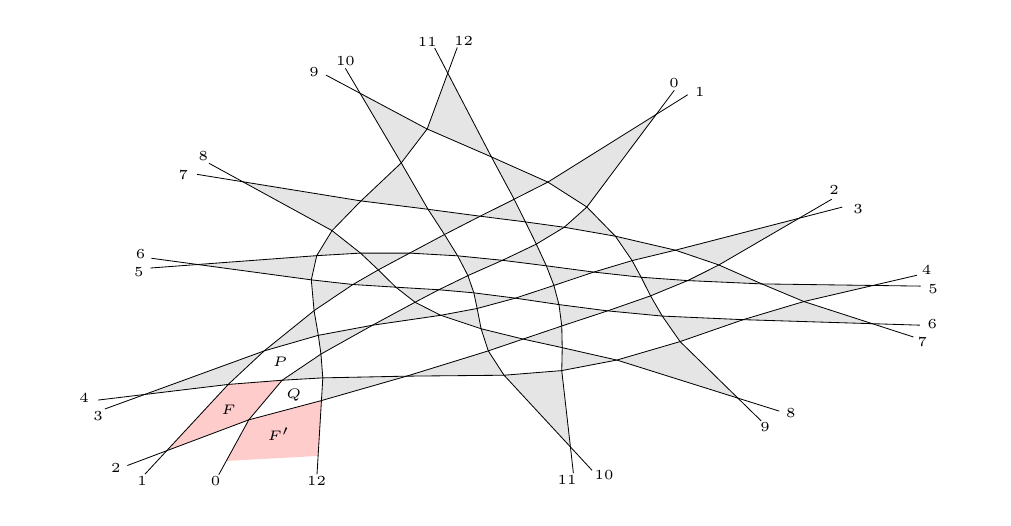
\begin{tikzpicture}[x=\linewidth,y=\linewidth,
  poly/.style={fill=gray!20},
  defect/.style={fill=red!20},
  ext/.style={black,line width=0.3pt},
  lbl/.style={inner sep=0pt,font=\tiny},
  plbl/.style={inner sep=0pt,font=\tiny}]
\useasboundingbox (0,0) rectangle (1,-0.89661);
\clip (0,0) rectangle (1,-0.89661);
\fill[poly] (0.76888,-0.48836) -- (0.88546,-0.49131) -- (0.81296,-0.52198) -- cycle;
\fill[poly] (0.67840,-0.42407) -- (0.80797,-0.36322) -- (0.72395,-0.45225) -- cycle;
\fill[poly] (0.69128,-0.48204) -- (0.72395,-0.45225) -- (0.76888,-0.48836) -- cycle;
\fill[poly] (0.74940,-0.55654) -- (0.81296,-0.52198) -- (0.88468,-0.56419) -- cycle;
\fill[poly] (0.66465,-0.54969) -- (0.74940,-0.55654) -- (0.68333,-0.59830) -- cycle;
\fill[poly] (0.64256,-0.47569) -- (0.69128,-0.48204) -- (0.65239,-0.51114) -- cycle;
\fill[poly] (0.61554,-0.39746) -- (0.67840,-0.42407) -- (0.63311,-0.44396) -- cycle;
\fill[poly] (0.54487,-0.29432) -- (0.65834,-0.16533) -- (0.58570,-0.34179) -- cycle;
\fill[poly] (0.56198,-0.38040) -- (0.58570,-0.34179) -- (0.61554,-0.39746) -- cycle;
\fill[poly] (0.59294,-0.46582) -- (0.63311,-0.44396) -- (0.64256,-0.47569) -- cycle;
\fill[poly] (0.60737,-0.53975) -- (0.65239,-0.51114) -- (0.66465,-0.54969) -- cycle;
\fill[poly] (0.61706,-0.63352) -- (0.68333,-0.59830) -- (0.74385,-0.70603) -- cycle;
\fill[poly] (0.55987,-0.60985) -- (0.61706,-0.63352) -- (0.55939,-0.65360) -- cycle;
\fill[poly] (0.55648,-0.52778) -- (0.60737,-0.53975) -- (0.55940,-0.56858) -- cycle;
\fill[poly] (0.54326,-0.45387) -- (0.59294,-0.46582) -- (0.55115,-0.49131) -- cycle;
\fill[poly] (0.52132,-0.37021) -- (0.56198,-0.38040) -- (0.53273,-0.41257) -- cycle;
\fill[poly] (0.48570,-0.24631) -- (0.54487,-0.29432) -- (0.50952,-0.32697) -- cycle;
\fill[poly] (0.47390,-0.35933) -- (0.50952,-0.32697) -- (0.52132,-0.37021) -- cycle;
\fill[poly] (0.49725,-0.44339) -- (0.53273,-0.41257) -- (0.54326,-0.45387) -- cycle;
\fill[poly] (0.51084,-0.51550) -- (0.55115,-0.49131) -- (0.55648,-0.52778) -- cycle;
\fill[poly] (0.51889,-0.59351) -- (0.55940,-0.56858) -- (0.55987,-0.60985) -- cycle;
\fill[poly] (0.49894,-0.66242) -- (0.55939,-0.65360) -- (0.56846,-0.79909) -- cycle;
\fill[poly] (0.47490,-0.57384) -- (0.51889,-0.59351) -- (0.48242,-0.61603) -- cycle;
\fill[poly] (0.46731,-0.50542) -- (0.51084,-0.51550) -- (0.47078,-0.53519) -- cycle;
\fill[poly] (0.45034,-0.43484) -- (0.49725,-0.44339) -- (0.46112,-0.47252) -- cycle;
\fill[poly] (0.41932,-0.34613) -- (0.47390,-0.35933) -- (0.43655,-0.39428) -- cycle;
\fill[poly] (0.40006,-0.42966) -- (0.43655,-0.39428) -- (0.45034,-0.43484) -- cycle;
\fill[poly] (0.43067,-0.49948) -- (0.46112,-0.47252) -- (0.46731,-0.50542) -- cycle;
\fill[poly] (0.43259,-0.54818) -- (0.47078,-0.53519) -- (0.47490,-0.57384) -- cycle;
\fill[poly] (0.38565,-0.49463) -- (0.43067,-0.49948) -- (0.40576,-0.52330) -- cycle;
\fill[poly] (0.34863,-0.42967) -- (0.40006,-0.42966) -- (0.36724,-0.46166) -- cycle;
\fill[poly] (0.34067,-0.48951) -- (0.36724,-0.46166) -- (0.38565,-0.49463) -- cycle;
\fill[poly] (0.36116,-0.56709) -- (0.40576,-0.52330) -- (0.43259,-0.54818) -- cycle;
\fill[poly] (0.39691,-0.66418) -- (0.48242,-0.61603) -- (0.49894,-0.66242) -- cycle;
\fill[poly] (0.30912,-0.66745) -- (0.39691,-0.66418) -- (0.30769,-0.71072) -- cycle;
\fill[poly] (0.30443,-0.58637) -- (0.36116,-0.56709) -- (0.30717,-0.62210) -- cycle;
\fill[poly] (0.29708,-0.48064) -- (0.34067,-0.48951) -- (0.29996,-0.53931) -- cycle;
\fill[poly] (0.31880,-0.38679) -- (0.34863,-0.42967) -- (0.30273,-0.43453) -- cycle;
\fill[poly] (0.39126,-0.25772) -- (0.41932,-0.34613) -- (0.34912,-0.33019) -- cycle;
\fill[poly] (0.44000,-0.08665) -- (0.48570,-0.24631) -- (0.41839,-0.19312) -- cycle;
\fill[poly] (0.34819,-0.12505) -- (0.41839,-0.19312) -- (0.39126,-0.25772) -- cycle;
\fill[poly] (0.22526,-0.29367) -- (0.34912,-0.33019) -- (0.31880,-0.38679) -- cycle;
\fill[poly] (0.17804,-0.45139) -- (0.30273,-0.43453) -- (0.29708,-0.48064) -- cycle;
\fill[poly] (0.24769,-0.61606) -- (0.29996,-0.53931) -- (0.30443,-0.58637) -- cycle;
\fill[poly] (0.26656,-0.67195) -- (0.30717,-0.62210) -- (0.30912,-0.66745) -- cycle;
\fill[poly] (0.12251,-0.69911) -- (0.24769,-0.61606) -- (0.21007,-0.67996) -- cycle;
\fill[defect] (0.14561,-0.80631) -- (0.21007,-0.67996) -- (0.26656,-0.67195) -- (0.23159,-0.74746) -- cycle;
\fill[defect] (0.23159,-0.74746) -- (0.30769,-0.71072) -- (0.30420,-0.81630) -- (0.20801,-0.82586) -- cycle;
\draw[ext] (0.67734,-0.11916) -- (0.65834,-0.16533) -- (0.58570,-0.34179) -- (0.56198,-0.38040) -- (0.53273,-0.41257) -- (0.49725,-0.44339) -- (0.46112,-0.47252) -- (0.43067,-0.49948) -- (0.40576,-0.52330) -- (0.36116,-0.56709) -- (0.30717,-0.62210) -- (0.26656,-0.67195) -- (0.23159,-0.74746) -- (0.20015,-0.85200);
\node[lbl] at (0.67713,-0.10511) {0};
\node[lbl] at (0.19669,-0.86349) {0};
\draw[ext] (0.69131,-0.12784) -- (0.65834,-0.16533) -- (0.54487,-0.29432) -- (0.50952,-0.32697) -- (0.47390,-0.35933) -- (0.43655,-0.39428) -- (0.40006,-0.42966) -- (0.36724,-0.46166) -- (0.34067,-0.48951) -- (0.29996,-0.53931) -- (0.24769,-0.61606) -- (0.21007,-0.67996) -- (0.14561,-0.80631) -- (0.12292,-0.85078);
\node[lbl] at (0.70400,-0.12179) {1};
\node[lbl] at (0.11977,-0.86349) {1};
\draw[ext] (0.84223,-0.32691) -- (0.80797,-0.36322) -- (0.72395,-0.45225) -- (0.69128,-0.48204) -- (0.65239,-0.51114) -- (0.60737,-0.53975) -- (0.55940,-0.56858) -- (0.51889,-0.59351) -- (0.48242,-0.61603) -- (0.39691,-0.66418) -- (0.30769,-0.71072) -- (0.23159,-0.74746) -- (0.14561,-0.80631) -- (0.10441,-0.83450);
\node[lbl] at (0.84471,-0.31023) {2};
\node[lbl] at (0.09221,-0.83926) {2};
\draw[ext] (0.85316,-0.34200) -- (0.80797,-0.36322) -- (0.67840,-0.42407) -- (0.63311,-0.44396) -- (0.59294,-0.46582) -- (0.55115,-0.49131) -- (0.51084,-0.51550) -- (0.47078,-0.53519) -- (0.43259,-0.54818) -- (0.36116,-0.56709) -- (0.30443,-0.58637) -- (0.24769,-0.61606) -- (0.12251,-0.69911) -- (0.08091,-0.72671);
\node[lbl] at (0.86978,-0.34484) {3};
\node[lbl] at (0.07380,-0.74017) {3};
\draw[ext] (0.93144,-0.47186) -- (0.88546,-0.49131) -- (0.81296,-0.52198) -- (0.74940,-0.55654) -- (0.68333,-0.59830) -- (0.61706,-0.63352) -- (0.55939,-0.65360) -- (0.49894,-0.66242) -- (0.39691,-0.66418) -- (0.30912,-0.66745) -- (0.26656,-0.67195) -- (0.21007,-0.67996) -- (0.12251,-0.69911) -- (0.07374,-0.70978);
\node[lbl] at (0.94164,-0.46270) {4};
\node[lbl] at (0.05913,-0.70551) {4};
\draw[ext] (0.93537,-0.49257) -- (0.88546,-0.49131) -- (0.76888,-0.48836) -- (0.69128,-0.48204) -- (0.64256,-0.47569) -- (0.59294,-0.46582) -- (0.54326,-0.45387) -- (0.49725,-0.44339) -- (0.45034,-0.43484) -- (0.40006,-0.42966) -- (0.34863,-0.42967) -- (0.30273,-0.43453) -- (0.17804,-0.45139) -- (0.12857,-0.45808);
\node[lbl] at (0.94822,-0.49736) {5};
\node[lbl] at (0.11636,-0.46545) {5};
\draw[ext] (0.93452,-0.56701) -- (0.88468,-0.56419) -- (0.74940,-0.55654) -- (0.66465,-0.54969) -- (0.60737,-0.53975) -- (0.55648,-0.52778) -- (0.51084,-0.51550) -- (0.46731,-0.50542) -- (0.43067,-0.49948) -- (0.38565,-0.49463) -- (0.34067,-0.48951) -- (0.29708,-0.48064) -- (0.17804,-0.45139) -- (0.12956,-0.43948);
\node[lbl] at (0.94756,-0.56419) {6};
\node[lbl] at (0.11821,-0.43084) {6};
\draw[ext] (0.92771,-0.58951) -- (0.88468,-0.56419) -- (0.81296,-0.52198) -- (0.76888,-0.48836) -- (0.72395,-0.45225) -- (0.67840,-0.42407) -- (0.61554,-0.39746) -- (0.56198,-0.38040) -- (0.52132,-0.37021) -- (0.47390,-0.35933) -- (0.41932,-0.34613) -- (0.34912,-0.33019) -- (0.22526,-0.29367) -- (0.17738,-0.27955);
\node[lbl] at (0.93699,-0.59908) {7};
\node[lbl] at (0.16316,-0.28074) {7};
\draw[ext] (0.78719,-0.73081) -- (0.74385,-0.70603) -- (0.61706,-0.63352) -- (0.55987,-0.60985) -- (0.51889,-0.59351) -- (0.47490,-0.57384) -- (0.43259,-0.54818) -- (0.40576,-0.52330) -- (0.38565,-0.49463) -- (0.36724,-0.46166) -- (0.34863,-0.42967) -- (0.31880,-0.38679) -- (0.22526,-0.29367) -- (0.18988,-0.25845);
\node[lbl] at (0.79937,-0.73503) {8};
\node[lbl] at (0.18409,-0.24540) {8};
\draw[ext] (0.76831,-0.74955) -- (0.74385,-0.70603) -- (0.68333,-0.59830) -- (0.66465,-0.54969) -- (0.65239,-0.51114) -- (0.64256,-0.47569) -- (0.63311,-0.44396) -- (0.61554,-0.39746) -- (0.58570,-0.34179) -- (0.54487,-0.29432) -- (0.48570,-0.24631) -- (0.41839,-0.19312) -- (0.34819,-0.12505) -- (0.31234,-0.09029);
\node[lbl] at (0.77242,-0.76176) {9};
\node[lbl] at (0.29993,-0.08431) {9};
\draw[ext] (0.59109,-0.84358) -- (0.56846,-0.79909) -- (0.49894,-0.66242) -- (0.48242,-0.61603) -- (0.47490,-0.57384) -- (0.47078,-0.53519) -- (0.46731,-0.50542) -- (0.46112,-0.47252) -- (0.45034,-0.43484) -- (0.43655,-0.39428) -- (0.41932,-0.34613) -- (0.39126,-0.25772) -- (0.34819,-0.12505) -- (0.33277,-0.07756);
\node[lbl] at (0.60380,-0.85230) {10};
\node[lbl] at (0.33286,-0.06378) {10};
\draw[ext] (0.57156,-0.84891) -- (0.56846,-0.79909) -- (0.55939,-0.65360) -- (0.55987,-0.60985) -- (0.55940,-0.56858) -- (0.55648,-0.52778) -- (0.55115,-0.49131) -- (0.54326,-0.45387) -- (0.53273,-0.41257) -- (0.52132,-0.37021) -- (0.50952,-0.32697) -- (0.48570,-0.24631) -- (0.44000,-0.08665) -- (0.42626,-0.03866);
\node[lbl] at (0.56504,-0.86287) {11};
\node[lbl] at (0.41856,-0.02729) {11};
\draw[ext] (0.30304,-0.85150) -- (0.30769,-0.71072) -- (0.30912,-0.66745) -- (0.30717,-0.62210) -- (0.30443,-0.58637) -- (0.29996,-0.53931) -- (0.29708,-0.48064) -- (0.30273,-0.43453) -- (0.31880,-0.38679) -- (0.34912,-0.33019) -- (0.39126,-0.25772) -- (0.41839,-0.19312) -- (0.44000,-0.08665) -- (0.44993,-0.03773);
\node[lbl] at (0.30264,-0.86349) {12};
\node[lbl] at (0.45671,-0.02580) {12};
\node[plbl] at (0.21029,-0.72843) {$F$};
\node[plbl] at (0.26287,-0.77509) {$F'$};
\node[plbl] at (0.27874,-0.69952) {$Q$};
\node[plbl] at (0.26448,-0.63713) {$P$};
\end{tikzpicture}

\caption{}
\end{subfigure}\hfill
\begin{subfigure}[c]{0.35\linewidth}% a third of the width of (a): the same scale
\centering
% Lower left cell of a 3x3 grid: a picture as wide as (a), clipped by 2/3 on the right and at the top.
\clipbox{0pt 0pt {0.65\width} {0.6\height}}{\begin{minipage}[b]{2.5\linewidth}% Generated by Visual Arnold
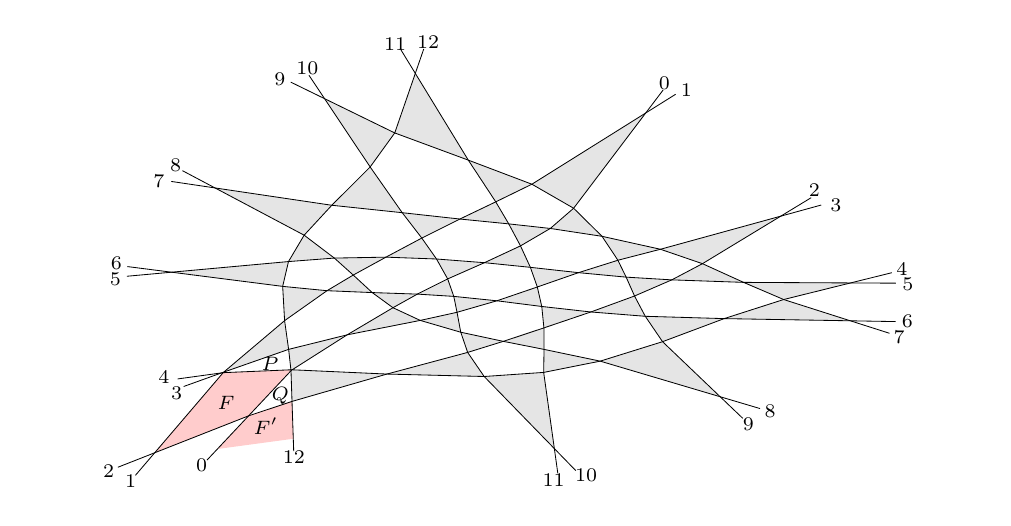
\begin{tikzpicture}[x=\linewidth,y=\linewidth,
  poly/.style={fill=gray!20},
  defect/.style={fill=red!20},
  ext/.style={black,line width=0.3pt},
  lbl/.style={inner sep=0pt,font=\scriptsize},
  plbl/.style={inner sep=0pt,font=\scriptsize}]
\useasboundingbox (0,0) rectangle (1,-0.89661);
\clip (0,0) rectangle (1,-0.89661);
\fill[poly] (0.74981,-0.48545) -- (0.86191,-0.48651) -- (0.79180,-0.51814) -- cycle;
\fill[poly] (0.66274,-0.42233) -- (0.78875,-0.35925) -- (0.70676,-0.44981) -- cycle;
\fill[poly] (0.67464,-0.48067) -- (0.70676,-0.44981) -- (0.74981,-0.48545) -- cycle;
\fill[poly] (0.72950,-0.55450) -- (0.79180,-0.51814) -- (0.86165,-0.55868) -- cycle;
\fill[poly] (0.64687,-0.55009) -- (0.72950,-0.55450) -- (0.66496,-0.59850) -- cycle;
\fill[poly] (0.62682,-0.47546) -- (0.67464,-0.48067) -- (0.63560,-0.51144) -- cycle;
\fill[poly] (0.60160,-0.39768) -- (0.66274,-0.42233) -- (0.61819,-0.44328) -- cycle;
\fill[poly] (0.52811,-0.29836) -- (0.64736,-0.16257) -- (0.57183,-0.34415) -- cycle;
\fill[poly] (0.54739,-0.38268) -- (0.57183,-0.34415) -- (0.60160,-0.39768) -- cycle;
\fill[poly] (0.57692,-0.46694) -- (0.61819,-0.44328) -- (0.62682,-0.47546) -- cycle;
\fill[poly] (0.58989,-0.54186) -- (0.63560,-0.51144) -- (0.64687,-0.55009) -- cycle;
\fill[poly] (0.59964,-0.63557) -- (0.66496,-0.59850) -- (0.72531,-0.70342) -- cycle;
\fill[poly] (0.54082,-0.61316) -- (0.59964,-0.63557) -- (0.54045,-0.65704) -- cycle;
\fill[poly] (0.53845,-0.53137) -- (0.58989,-0.54186) -- (0.54069,-0.57220) -- cycle;
\fill[poly] (0.52652,-0.45677) -- (0.57692,-0.46694) -- (0.53380,-0.49425) -- cycle;
\fill[poly] (0.50384,-0.37395) -- (0.54739,-0.38268) -- (0.51617,-0.41590) -- cycle;
\fill[poly] (0.46149,-0.25242) -- (0.52811,-0.29836) -- (0.49027,-0.33198) -- cycle;
\fill[poly] (0.45269,-0.36471) -- (0.49027,-0.33198) -- (0.50384,-0.37395) -- cycle;
\fill[poly] (0.47842,-0.44792) -- (0.51617,-0.41590) -- (0.52652,-0.45677) -- cycle;
\fill[poly] (0.49147,-0.52055) -- (0.53380,-0.49425) -- (0.53845,-0.53137) -- cycle;
\fill[poly] (0.49819,-0.59786) -- (0.54069,-0.57220) -- (0.54082,-0.61316) -- cycle;
\fill[poly] (0.47814,-0.66484) -- (0.54045,-0.65704) -- (0.55163,-0.80225) -- cycle;
\fill[poly] (0.45360,-0.58046) -- (0.49819,-0.59786) -- (0.46083,-0.61894) -- cycle;
\fill[poly] (0.44630,-0.51215) -- (0.49147,-0.52055) -- (0.44971,-0.54247) -- cycle;
\fill[poly] (0.42820,-0.44090) -- (0.47842,-0.44792) -- (0.43990,-0.47887) -- cycle;
\fill[poly] (0.39231,-0.35265) -- (0.45269,-0.36471) -- (0.41280,-0.40100) -- cycle;
\fill[poly] (0.37526,-0.43738) -- (0.41280,-0.40100) -- (0.42820,-0.44090) -- cycle;
\fill[poly] (0.40813,-0.50781) -- (0.43990,-0.47887) -- (0.44630,-0.51215) -- cycle;
\fill[poly] (0.41120,-0.55795) -- (0.44971,-0.54247) -- (0.45360,-0.58046) -- cycle;
\fill[poly] (0.36086,-0.50488) -- (0.40813,-0.50781) -- (0.38261,-0.53374) -- cycle;
\fill[poly] (0.32119,-0.43914) -- (0.37526,-0.43738) -- (0.34100,-0.47148) -- cycle;
\fill[poly] (0.31352,-0.50131) -- (0.34100,-0.47148) -- (0.36086,-0.50488) -- cycle;
\fill[poly] (0.33462,-0.58543) -- (0.38261,-0.53374) -- (0.41120,-0.55795) -- cycle;
\fill[poly] (0.37627,-0.66019) -- (0.46083,-0.61894) -- (0.47814,-0.66484) -- cycle;
\fill[poly] (0.27578,-0.65388) -- (0.27703,-0.65205) -- (0.37627,-0.66019) -- (0.27686,-0.71234) -- cycle;
\fill[poly] (0.27332,-0.61315) -- (0.33462,-0.58543) -- (0.27703,-0.65205) -- (0.27570,-0.65205) -- cycle;
\fill[poly] (0.26708,-0.49307) -- (0.31352,-0.50131) -- (0.26910,-0.55840) -- cycle;
\fill[poly] (0.28957,-0.39550) -- (0.32119,-0.43914) -- (0.27317,-0.44580) -- cycle;
\fill[poly] (0.35871,-0.26547) -- (0.39231,-0.35265) -- (0.31854,-0.33848) -- cycle;
\fill[poly] (0.40601,-0.08712) -- (0.46149,-0.25242) -- (0.38446,-0.20063) -- cycle;
\fill[poly] (0.31095,-0.13527) -- (0.38446,-0.20063) -- (0.35871,-0.26547) -- cycle;
\fill[poly] (0.19623,-0.30544) -- (0.31854,-0.33848) -- (0.28957,-0.39550) -- cycle;
\fill[poly] (0.15071,-0.46605) -- (0.27317,-0.44580) -- (0.26708,-0.49307) -- cycle;
\fill[poly] (0.20537,-0.65646) -- (0.26910,-0.55840) -- (0.27332,-0.61315) -- cycle;
\fill[poly] (0.20307,-0.65797) -- (0.20537,-0.65646) -- (0.20477,-0.65754) -- cycle;
\fill[defect] (0.13306,-0.81021) -- (0.20477,-0.65754) -- (0.27570,-0.65205) -- (0.27578,-0.65388) -- (0.23137,-0.73984) -- cycle;
\fill[defect] (0.23137,-0.73984) -- (0.27686,-0.71234) -- (0.27819,-0.78350) -- (0.19872,-0.80306) -- cycle;
\draw[ext] (0.66559,-0.11876) -- (0.64736,-0.16257) -- (0.57183,-0.34415) -- (0.54739,-0.38268) -- (0.51617,-0.41590) -- (0.47842,-0.44792) -- (0.43990,-0.47887) -- (0.40813,-0.50781) -- (0.38261,-0.53374) -- (0.33462,-0.58543) -- (0.27703,-0.65205) -- (0.27578,-0.65388) -- (0.23137,-0.73984) -- (0.18783,-0.82414);
\node[lbl] at (0.66692,-0.10565) {0};
\node[lbl] at (0.18232,-0.83480) {0};
\draw[ext] (0.67867,-0.12692) -- (0.64736,-0.16257) -- (0.52811,-0.29836) -- (0.49027,-0.33198) -- (0.45269,-0.36471) -- (0.41280,-0.40100) -- (0.37526,-0.43738) -- (0.34100,-0.47148) -- (0.31352,-0.50131) -- (0.26910,-0.55840) -- (0.20537,-0.65646) -- (0.20477,-0.65754) -- (0.13306,-0.81021) -- (0.11289,-0.85315);
\node[lbl] at (0.68987,-0.11995) {1};
\node[lbl] at (0.10779,-0.86401) {1};
\draw[ext] (0.82059,-0.32408) -- (0.78875,-0.35925) -- (0.70676,-0.44981) -- (0.67464,-0.48067) -- (0.63560,-0.51144) -- (0.58989,-0.54186) -- (0.54069,-0.57220) -- (0.49819,-0.59786) -- (0.46083,-0.61894) -- (0.37627,-0.66019) -- (0.27686,-0.71234) -- (0.23137,-0.73984) -- (0.13306,-0.81021) -- (0.09448,-0.83782);
\node[lbl] at (0.82400,-0.30907) {2};
\node[lbl] at (0.08472,-0.84481) {2};
\draw[ext] (0.83117,-0.33801) -- (0.78875,-0.35925) -- (0.66274,-0.42233) -- (0.61819,-0.44328) -- (0.57692,-0.46694) -- (0.53380,-0.49425) -- (0.49147,-0.52055) -- (0.44971,-0.54247) -- (0.41120,-0.55795) -- (0.33462,-0.58543) -- (0.27332,-0.61315) -- (0.20537,-0.65646) -- (0.20307,-0.65797) -- (0.16336,-0.68393);
\node[lbl] at (0.84655,-0.33875) {3};
\node[lbl] at (0.15609,-0.69684) {3};
\draw[ext] (0.90516,-0.46699) -- (0.86191,-0.48651) -- (0.79180,-0.51814) -- (0.72950,-0.55450) -- (0.66496,-0.59850) -- (0.59964,-0.63557) -- (0.54045,-0.65704) -- (0.47814,-0.66484) -- (0.37627,-0.66019) -- (0.27703,-0.65205) -- (0.27570,-0.65205) -- (0.20477,-0.65754) -- (0.20307,-0.65797) -- (0.15704,-0.66949);
\node[lbl] at (0.91556,-0.45956) {4};
\node[lbl] at (0.14263,-0.66607) {4};
\draw[ext] (0.90935,-0.48695) -- (0.86191,-0.48651) -- (0.74981,-0.48545) -- (0.67464,-0.48067) -- (0.62682,-0.47546) -- (0.57692,-0.46694) -- (0.52652,-0.45677) -- (0.47842,-0.44792) -- (0.42820,-0.44090) -- (0.37526,-0.43738) -- (0.32119,-0.43914) -- (0.27317,-0.44580) -- (0.15071,-0.46605) -- (0.10390,-0.47380);
\node[lbl] at (0.92188,-0.48957) {5};
\node[lbl] at (0.09195,-0.47922) {5};
\draw[ext] (0.90907,-0.56018) -- (0.86165,-0.55868) -- (0.72950,-0.55450) -- (0.64687,-0.55009) -- (0.58989,-0.54186) -- (0.53845,-0.53137) -- (0.49147,-0.52055) -- (0.44630,-0.51215) -- (0.40813,-0.50781) -- (0.36086,-0.50488) -- (0.31352,-0.50131) -- (0.26708,-0.49307) -- (0.15071,-0.46605) -- (0.10449,-0.45533);
\node[lbl] at (0.92147,-0.55916) {6};
\node[lbl] at (0.09291,-0.44914) {6};
\draw[ext] (0.90269,-0.58250) -- (0.86165,-0.55868) -- (0.79180,-0.51814) -- (0.74981,-0.48545) -- (0.70676,-0.44981) -- (0.66274,-0.42233) -- (0.60160,-0.39768) -- (0.54739,-0.38268) -- (0.50384,-0.37395) -- (0.45269,-0.36471) -- (0.39231,-0.35265) -- (0.31854,-0.33848) -- (0.19623,-0.30544) -- (0.15042,-0.29307);
\node[lbl] at (0.91267,-0.58992) {7};
\node[lbl] at (0.13738,-0.29252) {7};
\draw[ext] (0.76706,-0.72596) -- (0.72531,-0.70342) -- (0.59964,-0.63557) -- (0.54082,-0.61316) -- (0.49819,-0.59786) -- (0.45360,-0.58046) -- (0.41120,-0.55795) -- (0.38261,-0.53374) -- (0.36086,-0.50488) -- (0.34100,-0.47148) -- (0.32119,-0.43914) -- (0.28957,-0.39550) -- (0.19623,-0.30544) -- (0.16208,-0.27250);
\node[lbl] at (0.77762,-0.73166) {8};
\node[lbl] at (0.15491,-0.26159) {8};
\draw[ext] (0.74897,-0.74454) -- (0.72531,-0.70342) -- (0.66496,-0.59850) -- (0.64687,-0.55009) -- (0.63560,-0.51144) -- (0.62682,-0.47546) -- (0.61819,-0.44328) -- (0.60160,-0.39768) -- (0.57183,-0.34415) -- (0.52811,-0.29836) -- (0.46149,-0.25242) -- (0.38446,-0.20063) -- (0.31095,-0.13527) -- (0.27550,-0.10374);
\node[lbl] at (0.75495,-0.75494) {9};
\node[lbl] at (0.26413,-0.09739) {9};
\draw[ext] (0.57400,-0.84409) -- (0.55163,-0.80225) -- (0.47814,-0.66484) -- (0.46083,-0.61894) -- (0.45360,-0.58046) -- (0.44971,-0.54247) -- (0.44630,-0.51215) -- (0.43990,-0.47887) -- (0.42820,-0.44090) -- (0.41280,-0.40100) -- (0.39231,-0.35265) -- (0.35871,-0.26547) -- (0.31095,-0.13527) -- (0.29462,-0.09072);
\node[lbl] at (0.58494,-0.85313) {10};
\node[lbl] at (0.29289,-0.07782) {10};
\draw[ext] (0.55527,-0.84956) -- (0.55163,-0.80225) -- (0.54045,-0.65704) -- (0.54082,-0.61316) -- (0.54069,-0.57220) -- (0.53845,-0.53137) -- (0.53380,-0.49425) -- (0.52652,-0.45677) -- (0.51617,-0.41590) -- (0.50384,-0.37395) -- (0.49027,-0.33198) -- (0.46149,-0.25242) -- (0.40601,-0.08712) -- (0.39091,-0.04214);
\node[lbl] at (0.55091,-0.86306) {11};
\node[lbl] at (0.38484,-0.03091) {11};
\draw[ext] (0.27864,-0.80722) -- (0.27686,-0.71234) -- (0.27578,-0.65388) -- (0.27570,-0.65205) -- (0.27332,-0.61315) -- (0.26910,-0.55840) -- (0.26708,-0.49307) -- (0.27317,-0.44580) -- (0.28957,-0.39550) -- (0.31854,-0.33848) -- (0.35871,-0.26547) -- (0.38446,-0.20063) -- (0.40601,-0.08712) -- (0.41486,-0.04051);
\node[lbl] at (0.27886,-0.81922) {12};
\node[lbl] at (0.41935,-0.02857) {12};
\node[plbl] at (0.20787,-0.71589) {$F$};
\node[plbl] at (0.24946,-0.75968) {$F'$};
\node[plbl] at (0.26451,-0.70202) {$Q$};
\node[plbl] at (0.25387,-0.64106) {$P$};
\end{tikzpicture}
\end{minipage}}
\caption{}
\end{subfigure}

\bigskip
\begin{subfigure}[b]{0.64\linewidth}
\centering
% Generated by Visual Arnold
\begin{tikzpicture}[x=\linewidth,y=\linewidth,
  poly/.style={fill=gray!20},
  ext/.style={black,line width=0.3pt},
  aug/.style={r-line,thick,dashed,line cap=round,line join=round},
  lbl/.style={inner sep=0pt,font=\tiny},
  plbl/.style={inner sep=0pt,font=\tiny}]
\useasboundingbox (0,0) rectangle (1,-0.89661);
\clip (0,0) rectangle (1,-0.89661);
\fill[poly] (0.28788,-0.61586) -- (0.28704,-0.61674) -- (0.22615,-0.63819) -- (0.23248,-0.60140) -- cycle;
\fill[poly] (0.21818,-0.68450) -- (0.20908,-0.72890) -- (0.14683,-0.75509) -- cycle;
\fill[poly] (0.28704,-0.61674) -- (0.22615,-0.63819) -- (0.21818,-0.68450) -- cycle;
\fill[poly] (0.33611,-0.63206) -- (0.34090,-0.59745) -- (0.28878,-0.61612) -- cycle;
\fill[poly] (0.27433,-0.70255) -- (0.32980,-0.68052) -- (0.33589,-0.63368) -- cycle;
\fill[poly] (0.19316,-0.79579) -- (0.20908,-0.72890) -- (0.27433,-0.70255) -- cycle;
\fill[poly] (0.39922,-0.65253) -- (0.32980,-0.68052) -- (0.33589,-0.63368) -- (0.33708,-0.63238) -- cycle;
\fill[poly] (0.51349,-0.67078) -- (0.49313,-0.83391) -- (0.46492,-0.66751) -- cycle;
\fill[poly] (0.46168,-0.62576) -- (0.46492,-0.66751) -- (0.39922,-0.65253) -- cycle;
\fill[poly] (0.38529,-0.58133) -- (0.33708,-0.63238) -- (0.33611,-0.63206) -- (0.34090,-0.59745) -- cycle;
\fill[poly] (0.34948,-0.54519) -- (0.34090,-0.59745) -- (0.28878,-0.61612) -- (0.28788,-0.61586) -- cycle;
\fill[poly] (0.31345,-0.45604) -- (0.26110,-0.46265) -- (0.27265,-0.43402) -- cycle;
\fill[poly] (0.39163,-0.49606) -- (0.34948,-0.54519) -- (0.36381,-0.48266) -- cycle;
\fill[poly] (0.37498,-0.44905) -- (0.36381,-0.48266) -- (0.31345,-0.45604) -- cycle;
\fill[poly] (0.37852,-0.34117) -- (0.33945,-0.33091) -- (0.36685,-0.30133) -- cycle;
\fill[poly] (0.40342,-0.44775) -- (0.37498,-0.44905) -- (0.39466,-0.40509) -- cycle;
\fill[poly] (0.41782,-0.50733) -- (0.39163,-0.49606) -- (0.40942,-0.47584) -- cycle;
\fill[poly] (0.44181,-0.55967) -- (0.38529,-0.58133) -- (0.42863,-0.53576) -- cycle;
\fill[poly] (0.48809,-0.61307) -- (0.46168,-0.62576) -- (0.46219,-0.58647) -- cycle;
\fill[poly] (0.54872,-0.66663) -- (0.51349,-0.67078) -- (0.51763,-0.63942) -- cycle;
\fill[poly] (0.62575,-0.64301) -- (0.65607,-0.76714) -- (0.54872,-0.66663) -- cycle;
\fill[poly] (0.52362,-0.59442) -- (0.51763,-0.63942) -- (0.48809,-0.61307) -- cycle;
\fill[poly] (0.46452,-0.54984) -- (0.46219,-0.58647) -- (0.44181,-0.55967) -- cycle;
\fill[poly] (0.44540,-0.51826) -- (0.42863,-0.53576) -- (0.41782,-0.50733) -- cycle;
\fill[poly] (0.49220,-0.53624) -- (0.46452,-0.54984) -- (0.46641,-0.52630) -- cycle;
\fill[poly] (0.57048,-0.56808) -- (0.52362,-0.59442) -- (0.52841,-0.55088) -- cycle;
\fill[poly] (0.69690,-0.61587) -- (0.62575,-0.64301) -- (0.61583,-0.58604) -- cycle;
\fill[poly] (0.61103,-0.54377) -- (0.61583,-0.58604) -- (0.57048,-0.56808) -- cycle;
\fill[poly] (0.53112,-0.51520) -- (0.52841,-0.55088) -- (0.49220,-0.53624) -- cycle;
\fill[poly] (0.46860,-0.49459) -- (0.46641,-0.52630) -- (0.44540,-0.51826) -- cycle;
\fill[poly] (0.43331,-0.44918) -- (0.40942,-0.47584) -- (0.40342,-0.44775) -- cycle;
\fill[poly] (0.50009,-0.46326) -- (0.46860,-0.49459) -- (0.46969,-0.45503) -- cycle;
\fill[poly] (0.57465,-0.49252) -- (0.53112,-0.51520) -- (0.53280,-0.47515) -- cycle;
\fill[poly] (0.64783,-0.52007) -- (0.61103,-0.54377) -- (0.60792,-0.50582) -- cycle;
\fill[poly] (0.60541,-0.47904) -- (0.60792,-0.50582) -- (0.57465,-0.49252) -- cycle;
\fill[poly] (0.53396,-0.42747) -- (0.53280,-0.47515) -- (0.50009,-0.46326) -- cycle;
\fill[poly] (0.46922,-0.40935) -- (0.46969,-0.45503) -- (0.43331,-0.44918) -- cycle;
\fill[poly] (0.42379,-0.35265) -- (0.39466,-0.40509) -- (0.37852,-0.34117) -- cycle;
\fill[poly] (0.50140,-0.37508) -- (0.46922,-0.40935) -- (0.46734,-0.36438) -- cycle;
\fill[poly] (0.55707,-0.39942) -- (0.53396,-0.42747) -- (0.53516,-0.38829) -- cycle;
\fill[poly] (0.64582,-0.46511) -- (0.60541,-0.47904) -- (0.59846,-0.42638) -- cycle;
\fill[poly] (0.72059,-0.54208) -- (0.64783,-0.52007) -- (0.68006,-0.49821) -- cycle;
\fill[poly] (0.82136,-0.65345) -- (0.69690,-0.61587) -- (0.76564,-0.59266) -- cycle;
\fill[poly] (0.83661,-0.57246) -- (0.76564,-0.59266) -- (0.72059,-0.54208) -- cycle;
\fill[poly] (0.77528,-0.43054) -- (0.68006,-0.49821) -- (0.64582,-0.46511) -- cycle;
\fill[poly] (0.58475,-0.36026) -- (0.59846,-0.42638) -- (0.55707,-0.39942) -- cycle;
\fill[poly] (0.53698,-0.33968) -- (0.53516,-0.38829) -- (0.50140,-0.37508) -- cycle;
\fill[poly] (0.66559,-0.23201) -- (0.58475,-0.36026) -- (0.56854,-0.31126) -- cycle;
\fill[poly] (0.54000,-0.25003) -- (0.56854,-0.31126) -- (0.53698,-0.33968) -- cycle;
\fill[poly] (0.46252,-0.28266) -- (0.46734,-0.36438) -- (0.42379,-0.35265) -- cycle;
\fill[poly] (0.50398,-0.18630) -- (0.50444,-0.18708) -- (0.46252,-0.28266) -- (0.46051,-0.22404) -- cycle;
\fill[poly] (0.54331,-0.13892) -- (0.54000,-0.25003) -- (0.50444,-0.18708) -- (0.50522,-0.18503) -- cycle;
\fill[poly] (0.54320,-0.07001) -- (0.50522,-0.18503) -- (0.54331,-0.13892) -- cycle;
\fill[poly] (0.45648,-0.10528) -- (0.46051,-0.22404) -- (0.50398,-0.18630) -- cycle;
\draw[ext] (0.66527,-0.80482) -- (0.65607,-0.76714) -- (0.62575,-0.64301) -- (0.61583,-0.58604) -- (0.61103,-0.54377) -- (0.60792,-0.50582) -- (0.60541,-0.47904) -- (0.59846,-0.42638) -- (0.58475,-0.36026) -- (0.56854,-0.31126) -- (0.54000,-0.25003) -- (0.50444,-0.18708) -- (0.50398,-0.18630) -- (0.45648,-0.10528) -- (0.43686,-0.07183);
\node[lbl] at (0.66687,-0.81721) {9};
\node[lbl] at (0.42629,-0.06278) {9};
\draw[ext] (0.49961,-0.87215) -- (0.49313,-0.83391) -- (0.46492,-0.66751) -- (0.46168,-0.62576) -- (0.46219,-0.58647) -- (0.46452,-0.54984) -- (0.46641,-0.52630) -- (0.46860,-0.49459) -- (0.46969,-0.45503) -- (0.46922,-0.40935) -- (0.46734,-0.36438) -- (0.46252,-0.28266) -- (0.46051,-0.22404) -- (0.45648,-0.10528) -- (0.45516,-0.06652);
\node[lbl] at (0.51369,-0.88394) {10};
\node[lbl] at (0.45925,-0.05323) {10};
\draw[ext] (0.48832,-0.87240) -- (0.49313,-0.83391) -- (0.51349,-0.67078) -- (0.51763,-0.63942) -- (0.52362,-0.59442) -- (0.52841,-0.55088) -- (0.53112,-0.51520) -- (0.53280,-0.47515) -- (0.53396,-0.42747) -- (0.53516,-0.38829) -- (0.53698,-0.33968) -- (0.54000,-0.25003) -- (0.54331,-0.13892) -- (0.54320,-0.07001) -- (0.54314,-0.03122);
\node[lbl] at (0.47476,-0.88435) {11};
\node[lbl] at (0.53187,-0.01874) {11};
\draw[ext] (0.32481,-0.71898) -- (0.32980,-0.68052) -- (0.33589,-0.63368) -- (0.33611,-0.63206) -- (0.34090,-0.59745) -- (0.34948,-0.54519) -- (0.36381,-0.48266) -- (0.37498,-0.44905) -- (0.39466,-0.40509) -- (0.42379,-0.35265) -- (0.46252,-0.28266) -- (0.50444,-0.18708) -- (0.50522,-0.18503) -- (0.54320,-0.07001) -- (0.55537,-0.03318);
\node[lbl] at (0.32326,-0.73088) {12};
\node[lbl] at (0.57038,-0.02226) {12};
\draw[aug] (0.18419,-0.83352) -- (0.19316,-0.79579) -- (0.20908,-0.72890) -- (0.21818,-0.68450) -- (0.22615,-0.63819) -- (0.23248,-0.60140) -- (0.26110,-0.46265) -- (0.27265,-0.43402) -- (0.33945,-0.33091) -- (0.36685,-0.30133) -- (0.46051,-0.22404) -- (0.50398,-0.18630) -- (0.50522,-0.18503) -- (0.54331,-0.13892) -- (0.56802,-0.10902);
\node[lbl] at (0.18724,-0.84820) {13};
\node[lbl] at (0.57566,-0.09976) {13};
\draw[ext] (0.16770,-0.82505) -- (0.19316,-0.79579) -- (0.27433,-0.70255) -- (0.33589,-0.63368) -- (0.33708,-0.63238) -- (0.38529,-0.58133) -- (0.42863,-0.53576) -- (0.44540,-0.51826) -- (0.46860,-0.49459) -- (0.50009,-0.46326) -- (0.53396,-0.42747) -- (0.55707,-0.39942) -- (0.58475,-0.36026) -- (0.66559,-0.23201) -- (0.68627,-0.19920);
\node[lbl] at (0.15399,-0.83110) {0};
\node[lbl] at (0.68530,-0.18255) {0};
\draw[ext] (0.11926,-0.78237) -- (0.14683,-0.75509) -- (0.21818,-0.68450) -- (0.28704,-0.61674) -- (0.28788,-0.61586) -- (0.34948,-0.54519) -- (0.39163,-0.49606) -- (0.40942,-0.47584) -- (0.43331,-0.44918) -- (0.46922,-0.40935) -- (0.50140,-0.37508) -- (0.53698,-0.33968) -- (0.56854,-0.31126) -- (0.66559,-0.23201) -- (0.69563,-0.20748);
\node[lbl] at (0.11694,-0.80010) {1};
\node[lbl] at (0.71228,-0.20639) {1};
\draw[ext] (0.11108,-0.77014) -- (0.14683,-0.75509) -- (0.20908,-0.72890) -- (0.27433,-0.70255) -- (0.32980,-0.68052) -- (0.39922,-0.65253) -- (0.46168,-0.62576) -- (0.48809,-0.61307) -- (0.52362,-0.59442) -- (0.57048,-0.56808) -- (0.61103,-0.54377) -- (0.64783,-0.52007) -- (0.68006,-0.49821) -- (0.77528,-0.43054) -- (0.80689,-0.40807);
\node[lbl] at (0.09381,-0.76550) {2};
\node[lbl] at (0.81245,-0.39214) {2};
\draw[ext] (0.18957,-0.65108) -- (0.22615,-0.63819) -- (0.28704,-0.61674) -- (0.28878,-0.61612) -- (0.34090,-0.59745) -- (0.38529,-0.58133) -- (0.44181,-0.55967) -- (0.46452,-0.54984) -- (0.49220,-0.53624) -- (0.53112,-0.51520) -- (0.57465,-0.49252) -- (0.60541,-0.47904) -- (0.64582,-0.46511) -- (0.77528,-0.43054) -- (0.81275,-0.42053);
\node[lbl] at (0.17825,-0.65507) {3};
\node[lbl] at (0.82856,-0.42642) {3};
\draw[ext] (0.19495,-0.59160) -- (0.23248,-0.60140) -- (0.28788,-0.61586) -- (0.28878,-0.61612) -- (0.33611,-0.63206) -- (0.33708,-0.63238) -- (0.39922,-0.65253) -- (0.46492,-0.66751) -- (0.51349,-0.67078) -- (0.54872,-0.66663) -- (0.62575,-0.64301) -- (0.69690,-0.61587) -- (0.76564,-0.59266) -- (0.83661,-0.57246) -- (0.87392,-0.56185);
\node[lbl] at (0.18334,-0.58857) {4};
\node[lbl] at (0.88542,-0.55428) {4};
\draw[ext] (0.22263,-0.46751) -- (0.26110,-0.46265) -- (0.31345,-0.45604) -- (0.37498,-0.44905) -- (0.40342,-0.44775) -- (0.43331,-0.44918) -- (0.46969,-0.45503) -- (0.50009,-0.46326) -- (0.53280,-0.47515) -- (0.57465,-0.49252) -- (0.60792,-0.50582) -- (0.64783,-0.52007) -- (0.72059,-0.54208) -- (0.83661,-0.57246) -- (0.87413,-0.58229);
\node[lbl] at (0.21072,-0.46902) {5};
\node[lbl] at (0.88578,-0.58962) {5};
\draw[ext] (0.23852,-0.41560) -- (0.27265,-0.43402) -- (0.31345,-0.45604) -- (0.36381,-0.48266) -- (0.39163,-0.49606) -- (0.41782,-0.50733) -- (0.44540,-0.51826) -- (0.46641,-0.52630) -- (0.49220,-0.53624) -- (0.52841,-0.55088) -- (0.57048,-0.56808) -- (0.61583,-0.58604) -- (0.69690,-0.61587) -- (0.82136,-0.65345) -- (0.85849,-0.66465);
\node[lbl] at (0.22796,-0.40990) {6};
\node[lbl] at (0.87399,-0.66172) {6};
\draw[ext] (0.30194,-0.32106) -- (0.33945,-0.33091) -- (0.37852,-0.34117) -- (0.42379,-0.35265) -- (0.46734,-0.36438) -- (0.50140,-0.37508) -- (0.53516,-0.38829) -- (0.55707,-0.39942) -- (0.59846,-0.42638) -- (0.64582,-0.46511) -- (0.68006,-0.49821) -- (0.72059,-0.54208) -- (0.76564,-0.59266) -- (0.82136,-0.65345) -- (0.84756,-0.68204);
\node[lbl] at (0.29033,-0.31801) {7};
\node[lbl] at (0.85164,-0.69729) {7};
\draw[ext] (0.35595,-0.26411) -- (0.36685,-0.30133) -- (0.37852,-0.34117) -- (0.39466,-0.40509) -- (0.40342,-0.44775) -- (0.40942,-0.47584) -- (0.41782,-0.50733) -- (0.42863,-0.53576) -- (0.44181,-0.55967) -- (0.46219,-0.58647) -- (0.48809,-0.61307) -- (0.51763,-0.63942) -- (0.54872,-0.66663) -- (0.65607,-0.76714) -- (0.68438,-0.79365);
\node[lbl] at (0.35258,-0.25259) {8};
\node[lbl] at (0.69439,-0.80112) {8};
\end{tikzpicture}

\caption{}
\end{subfigure}
\caption{Collapse augmentation. (a) The original arrangement. $F$ and $F'$ are the internal and the external defect. Next to them are the white quadrilateral $Q$ and the pentagon $P$. (b) The triangles with vertices at the endpoints of the common side of $P$ and $F$ are collapsed into triple points. Then $P$ and $Q$ become triangles. The common triple point of $P$ and $Q$ is already surrounded by four triangles, and the other triple point by only three. The third of these triangles is projective, bounded by pseudolines $3,4,\infty$. (c) Pseudoline 13 is added so that the second triple point gets a fourth triangle, bounded by pseudolines $1,3,13$. The resulting arrangement of 14 pseudolines has $a_3=54$ triangles and a third triple point.}
\label{fig:collapse}
\end{figure}

\subsection{Augmentation algorithm}

We wrote a program that adds one pseudoline to an arrangement in all possible ways to reach $a_3\ge K$ for a given $K$, by default \eqref{eq:conj-bound}. The source code and the output words are published in the repository~\cite{nonsimple-arrangements}. The new pseudoline follows a route through the faces of the projective closure and crosses each pseudoline once. It leaves a face through a side or through a simple vertex, which then becomes a triple point.
Working in the projective closure lets the program treat external defects as quadrilaterals, as both patterns require.

Augmentation patterns restrict the routes. For direct augmentation, the route must pass through a defect. For collapse augmentation, the program first finds suitable triangles to turn into triple points, and the route must cut off a triangle at the triple point surrounded by three triangles. If there are no quadrilateral defects, all routes are searched, including the outermost line.
The search has two stages. A dynamic program over the faces bounds from above, for every affine chart simultaneously, the number of triangles that a route can give. Then a depth-first search enumerates the routes, pruned by this bound.

After the new pseudoline has been drawn, the program tests all affine charts (that is, all choices of the pseudoline of the projective arrangement that goes to infinity) and looks for one in which $a_3\ge K$.
If the pseudoline sent to infinity passes through a triple point, the other two pseudolines of the point do not cross in the affine chart, like parallel lines. Such charts are allowed.

Because of the projective nature of the computations, it is enough to take as input one representative of each projective equivalence class ($P$-class,~\cite[Definition~5.8]{pu26b}), not all affine arrangements with an odd number of pseudolines.
For every input and every route found, the program emits one word, in an affine chart where $a_3\ge K$.

\subsection{Computational results}

In~\cite{pu26b} we obtained exhaustive enumerations of 2-defective arrangements for $n\equiv1\pmod 6$ with $n=7,13,19$, and of perfect arrangements for $n\le27$. As input we took the representatives of their $P$-classes~\cite[Subsection~7.2]{pu26b}. The results for 2-defective inputs are summarized in \cref{tab:augmentation}.

\begin{table}[tb]
\centering
\caption{Augmentation of 2-defective arrangements, by $P$-classes. The target $a_3$ is the bound \eqref{eq:conj-bound}; an input is productive if at least one of its augmentations reaches it.}
\label{tab:augmentation}
\begin{tabular}{lrrrrrrrr}
\toprule
 & & & \multicolumn{3}{c}{productive inputs} & \multicolumn{3}{c}{output $P$-classes} \\
\cmidrule(lr){4-6}\cmidrule(lr){7-9}
$n\to N$ & $a_3$ & inputs & direct & collapse & total & direct & collapse & total \\
\midrule
$7\to8$   & 15  & 1    & 1  & 1  & 1   & 1   & 1   & 1   \\
$13\to14$ & 54  & 6    & 3  & 2  & 4   & 10  & 4   & 14  \\
$19\to20$ & 117 & 1312 & 64 & 75 & 137 & 275 & 168 & 443 \\
\bottomrule
\end{tabular}
\end{table}

At $n=7$ the single input class is productive under both patterns, and they give the same output $P$-class.
At $n=13$ one of the four productive input classes is productive under both patterns, and at $n=19$ two of the 137.
At $N=14,20$ the patterns share no output class: each of the 14 output classes at $N=14$ and each of the 443 at $N=20$ comes from exactly one input class by exactly one pattern.
For many input arrangements, the program finds no route that reaches \eqref{eq:conj-bound}.\footnote{Consider direct augmentation.
To exceed \eqref{eq:blanc-even}, the new pseudoline must pass through vertices of the original arrangement, which are all simple, so it creates triple points.
At least one of them must be reduced: otherwise, by \cref{lem:perturbation}, the triple points can be removed without losing triangles, and the result is a simple arrangement.
A reduced triple point is an endpoint of double segments (\cref{sec:segment-count}). Unused and double segments form the phase seam, which contains a closed curve that is non-contractible in $\mathbb{RP}^2$ (\cref{lem:seam}; \cref{fig:phase-seam} shows it for an arrangement obtained by direct augmentation).
The local coloring differs from the checkerboard coloring of the original arrangement only in the faces cut by the new pseudoline, so the seam lies within these faces and runs along the new pseudoline, which is non-contractible as well.
% The reduced triple points lie on both.
We expect the criterion for reaching \eqref{eq:conj-bound} to lie in the relative position of these two curves, but we have not found it.}
For larger $n$, augmentation also reaches \eqref{eq:conj-bound}: we found examples at $n=25,31,37,43$~\cite{nonsimple-arrangements}.

As mentioned above, a 2-defective arrangement may contain one pentagonal defect. Such arrangements first appear at $n=25$. For all 2324 $P$-classes of such arrangements of 25 pseudolines, the program finds no augmentation reaching \eqref{eq:conj-bound}.

Applied to perfect arrangements, the program produces simple and non-simple arrangements, but none exceeds \eqref{eq:blanc-even}: multiple points give no advantage there.

Both augmentation patterns work for pseudolines and do not guarantee stretchability.
We stretched all 14 augmented $P$-classes for $N=14$, 353 of the 443 for $N=20$, and 25 for $N=32$; they are published in the online gallery~\cite{gallery}.
Some of them contain a pair of parallel lines; a small rotation of one line of the pair  makes them cross without decreasing the number of triangles.
Examples are shown in \cref{fig:n20,fig:n20-collapse,fig:n32}, and an arrangement of 44 pseudolines in \cref{fig:n44}.

Augmentation does not produce all known optima. A new pseudoline added to 9 pseudolines creates at most 4 triple points, and collapse adds at most 2, so the arrangements with $N=10$ and 10 triple points (\cref{fig:n10}) cannot be obtained this way. For $N=12$, there is no perfect arrangement of 11 pseudolines, and for the optimal arrangements of 11 pseudolines the program finds no augmentation reaching \eqref{eq:conj-bound}; all optima for $N=12$ are non-simple (\cref{tab:triple-points}).
